% Options for packages loaded elsewhere
\PassOptionsToPackage{unicode}{hyperref}
\PassOptionsToPackage{hyphens}{url}
\PassOptionsToPackage{dvipsnames,svgnames,x11names}{xcolor}
%
\documentclass[
]{agujournal2019}

\usepackage{amsmath,amssymb}
\usepackage{iftex}
\ifPDFTeX
  \usepackage[T1]{fontenc}
  \usepackage[utf8]{inputenc}
  \usepackage{textcomp} % provide euro and other symbols
\else % if luatex or xetex
  \usepackage{unicode-math}
  \defaultfontfeatures{Scale=MatchLowercase}
  \defaultfontfeatures[\rmfamily]{Ligatures=TeX,Scale=1}
\fi
\usepackage{lmodern}
\ifPDFTeX\else  
    % xetex/luatex font selection
\fi
% Use upquote if available, for straight quotes in verbatim environments
\IfFileExists{upquote.sty}{\usepackage{upquote}}{}
\IfFileExists{microtype.sty}{% use microtype if available
  \usepackage[]{microtype}
  \UseMicrotypeSet[protrusion]{basicmath} % disable protrusion for tt fonts
}{}
\makeatletter
\@ifundefined{KOMAClassName}{% if non-KOMA class
  \IfFileExists{parskip.sty}{%
    \usepackage{parskip}
  }{% else
    \setlength{\parindent}{0pt}
    \setlength{\parskip}{6pt plus 2pt minus 1pt}}
}{% if KOMA class
  \KOMAoptions{parskip=half}}
\makeatother
\usepackage{xcolor}
\setlength{\emergencystretch}{3em} % prevent overfull lines
\setcounter{secnumdepth}{5}
% Make \paragraph and \subparagraph free-standing
\makeatletter
\ifx\paragraph\undefined\else
  \let\oldparagraph\paragraph
  \renewcommand{\paragraph}{
    \@ifstar
      \xxxParagraphStar
      \xxxParagraphNoStar
  }
  \newcommand{\xxxParagraphStar}[1]{\oldparagraph*{#1}\mbox{}}
  \newcommand{\xxxParagraphNoStar}[1]{\oldparagraph{#1}\mbox{}}
\fi
\ifx\subparagraph\undefined\else
  \let\oldsubparagraph\subparagraph
  \renewcommand{\subparagraph}{
    \@ifstar
      \xxxSubParagraphStar
      \xxxSubParagraphNoStar
  }
  \newcommand{\xxxSubParagraphStar}[1]{\oldsubparagraph*{#1}\mbox{}}
  \newcommand{\xxxSubParagraphNoStar}[1]{\oldsubparagraph{#1}\mbox{}}
\fi
\makeatother


\providecommand{\tightlist}{%
  \setlength{\itemsep}{0pt}\setlength{\parskip}{0pt}}\usepackage{longtable,booktabs,array}
\usepackage{calc} % for calculating minipage widths
% Correct order of tables after \paragraph or \subparagraph
\usepackage{etoolbox}
\makeatletter
\patchcmd\longtable{\par}{\if@noskipsec\mbox{}\fi\par}{}{}
\makeatother
% Allow footnotes in longtable head/foot
\IfFileExists{footnotehyper.sty}{\usepackage{footnotehyper}}{\usepackage{footnote}}
\makesavenoteenv{longtable}
\usepackage{graphicx}
\makeatletter
\def\maxwidth{\ifdim\Gin@nat@width>\linewidth\linewidth\else\Gin@nat@width\fi}
\def\maxheight{\ifdim\Gin@nat@height>\textheight\textheight\else\Gin@nat@height\fi}
\makeatother
% Scale images if necessary, so that they will not overflow the page
% margins by default, and it is still possible to overwrite the defaults
% using explicit options in \includegraphics[width, height, ...]{}
\setkeys{Gin}{width=\maxwidth,height=\maxheight,keepaspectratio}
% Set default figure placement to htbp
\makeatletter
\def\fps@figure{htbp}
\makeatother
% definitions for citeproc citations
\NewDocumentCommand\citeproctext{}{}
\NewDocumentCommand\citeproc{mm}{%
  \begingroup\def\citeproctext{#2}\cite{#1}\endgroup}
\makeatletter
 % allow citations to break across lines
 \let\@cite@ofmt\@firstofone
 % avoid brackets around text for \cite:
 \def\@biblabel#1{}
 \def\@cite#1#2{{#1\if@tempswa , #2\fi}}
\makeatother
\newlength{\cslhangindent}
\setlength{\cslhangindent}{1.5em}
\newlength{\csllabelwidth}
\setlength{\csllabelwidth}{3em}
\newenvironment{CSLReferences}[2] % #1 hanging-indent, #2 entry-spacing
 {\begin{list}{}{%
  \setlength{\itemindent}{0pt}
  \setlength{\leftmargin}{0pt}
  \setlength{\parsep}{0pt}
  % turn on hanging indent if param 1 is 1
  \ifodd #1
   \setlength{\leftmargin}{\cslhangindent}
   \setlength{\itemindent}{-1\cslhangindent}
  \fi
  % set entry spacing
  \setlength{\itemsep}{#2\baselineskip}}}
 {\end{list}}
\usepackage{calc}
\newcommand{\CSLBlock}[1]{\hfill\break\parbox[t]{\linewidth}{\strut\ignorespaces#1\strut}}
\newcommand{\CSLLeftMargin}[1]{\parbox[t]{\csllabelwidth}{\strut#1\strut}}
\newcommand{\CSLRightInline}[1]{\parbox[t]{\linewidth - \csllabelwidth}{\strut#1\strut}}
\newcommand{\CSLIndent}[1]{\hspace{\cslhangindent}#1}

\usepackage{url} %this package should fix any errors with URLs in refs.
\usepackage{lineno}
\usepackage[inline]{trackchanges} %for better track changes. finalnew option will compile document with changes incorporated.
\usepackage{soul}
\linenumbers
\makeatletter
\@ifpackageloaded{caption}{}{\usepackage{caption}}
\AtBeginDocument{%
\ifdefined\contentsname
  \renewcommand*\contentsname{Table of contents}
\else
  \newcommand\contentsname{Table of contents}
\fi
\ifdefined\listfigurename
  \renewcommand*\listfigurename{List of Figures}
\else
  \newcommand\listfigurename{List of Figures}
\fi
\ifdefined\listtablename
  \renewcommand*\listtablename{List of Tables}
\else
  \newcommand\listtablename{List of Tables}
\fi
\ifdefined\figurename
  \renewcommand*\figurename{Figure}
\else
  \newcommand\figurename{Figure}
\fi
\ifdefined\tablename
  \renewcommand*\tablename{Table}
\else
  \newcommand\tablename{Table}
\fi
}
\@ifpackageloaded{float}{}{\usepackage{float}}
\floatstyle{ruled}
\@ifundefined{c@chapter}{\newfloat{codelisting}{h}{lop}}{\newfloat{codelisting}{h}{lop}[chapter]}
\floatname{codelisting}{Listing}
\newcommand*\listoflistings{\listof{codelisting}{List of Listings}}
\makeatother
\makeatletter
\makeatother
\makeatletter
\@ifpackageloaded{caption}{}{\usepackage{caption}}
\@ifpackageloaded{subcaption}{}{\usepackage{subcaption}}
\makeatother

\ifLuaTeX
  \usepackage{selnolig}  % disable illegal ligatures
\fi
\usepackage{bookmark}

\IfFileExists{xurl.sty}{\usepackage{xurl}}{} % add URL line breaks if available
\urlstyle{same} % disable monospaced font for URLs
\hypersetup{
  pdftitle={Cumulative and component impacts of the human footprint on remotely sensed biodiversity indicators using dissimilarity to high integrity reference states.},
  pdfauthor={Evan Muise; Nicholas Coops; Txomin Hermosilla; Christopher Mulverhill; Cole Burton; Stephen Ban},
  pdfkeywords={Protected areas, Coarsened exact matching, Reference
states, Remote sensing, Ecosystem structure, Ecosystem
function, Anthropogenic pressure, Human footprint},
  colorlinks=true,
  linkcolor={blue},
  filecolor={Maroon},
  citecolor={Blue},
  urlcolor={Blue},
  pdfcreator={LaTeX via pandoc}}



\draftfalse

\begin{document}
\title{Cumulative and component impacts of the human footprint on
remotely sensed biodiversity indicators using dissimilarity to high
integrity reference states.}

\authors{Evan Muise\affil{1}, Nicholas Coops\affil{1}, Txomin
Hermosilla\affil{2}, Christopher Mulverhill\affil{1}, Cole
Burton\affil{1}, Stephen Ban\affil{3}}
\affiliation{1}{Department of Forest Resource Management, University of
British Columbia, Vancouver, British Columbia,
Canada, }\affiliation{2}{Canadian Forest Service (Pacific Forestry
Centre), Natural Resources Canada, Victoria, British Columbia,
Canada, }\affiliation{3}{BC Parks, Government of British Columbia,
Victoria, British Columbia, Canada, }
\correspondingauthor{Evan Muise}{evanmuis@student.ubc.ca}







\textbf{Abstract}

Forests with high ecological integrity are fundamental for biodiversity
conservation, and provide integral ecosystem services. These forests
have natural or near-natural ecosystem structure, function, and
composition. Anthropogenic pressures such as habitat loss,
overexploitation of natural resources, and land use changes are leading
to the degradation or loss of high-integrity forests. As a result,
assessing forest integrity over large areas is increasingly important
for a range of conservation initiatives. In this study, we used remote
sensing-derived forest structural and functioning metrics alongside a
high-quality reference state to calculate ecological dissimilarity as a
proxy for ecological integrity. We examined stand-level integrity and
focused on forest structural attributes such as canopy height, cover,
complexity, and biomass, as well as the Dynamic Habitat Indices, which
summarize annual energy availability relevant for biodiversity. We
further refined our reference states by using coarsened exact matching
to ensure our comparisons were drawn from suitable protected analogs. We
applied these methods to Vancouver Island, Canada, where we assessed the
distance, in structural and functional space, to matched high-integrity
forests found in the island's oldest and largest protected area. We also
assessed how individual and cumulative anthropogenic pressure affect the
ecological integrity of forests on the island. We found that mean forest
structural dissimilarity increased from 0.11 to 0.24 under high levels
of anthropogenic pressure (ANOVA; p \textless{} 0.01), while functional
dissimilarity was not impacted by any anthropogenic pressure (ANOVA; p
\textgreater{} 0.05). This indicates that anthropogenic pressures were
observed to directly influence forest canopy characteristics, and less
so energy availability. For individual pressures, we found that built
environments, harvesting, and population density influenced structural
dissimilarity (ANOVA; p \textless{} 0.05), while roads did not influence
structural dissimilarity (ANOVA; p \textgreater{} 0.05). These methods
for identifying high-integrity forests can be used to identify areas to
be prioritized for protection or restoration, which in turn progresses
towards the Kunming-Montreal Global Biodiversity Framework's goal of
30\% of all ecosystems protected, while focusing on high-integrity
ecosystems.

\newpage

\section{Introduction}\label{introduction}

Forests contain large amounts of biodiversity (Cardinale et al., 2012;
Myers, 1988) and provide important ecosystem services, including
nutrient cycling, carbon sequestration, timber, recreation areas, among
others (Thompson et al., 2009). However, the ongoing impact of
anthropogenic pressures such as climate change, overexploitation of
natural resources, and invasive species are leading to forest
degradation and reducing the ability of forested ecosystems to provide
these services (Grantham et al., 2020). Therefore it is imperative to
maintain and conserve forests that have high ecological integrity, as
defined by natural or near-natural levels of forest structure, function,
and composition (Hansen et al., 2021). The importance of high-integrity
ecosystems has led to a general call to move beyond simple
quantification of ecosystem or forest extent in conservation strategies
to other metrics which additionally consider the integrity of the
conserved ecosystem (Ferrier et al., 2024; Hansen et al., 2020; Muise et
al., 2022). In December 2022, the Kunming-Montreal Global Biodiversity
Framework (GBF) was adopted with the goal of restoring and safeguarding
global biodiversity (Convention on Biological Diversity, 2023). Targets
within this framework include restoring 30\% of all degraded ecosystems,
protecting 30\% of the Earth's terrestrial, inland water, and marine
areas by 2030, and achieving no loss of high biodiversity importance
areas, especially high ecological integrity ecosystems (Convention on
Biological Diversity, 2023). However, there are currently no spatially
explicitly assessments of ecological integrity available at broad
spatial scales, making progress towards these goals difficult to
quantify.

Assessing ecological integrity requires a comprehensive evaluation of
ecosystem structure, function, and composition, which can be effectively
achieved using remote sensing-derived indicators (Pereira et al., 2013;
Skidmore et al., 2021). Advances in remote sensing technologies such as
light detection and ranging (lidar) allow accurate measurement of forest
structural attributes, including canopy height, canopy cover, vertical
complexity, and biomass (Bergen et al., 2009; Valbuena et al., 2020).
These indicators of forest structure can provide critical insights into
habitat quality and the ability of ecosystems to support biodiversity
(Gao et al., 2014; Guo et al., 2017; Macarthur and Macarthur, 1961), and
are rapidly becoming available at national scales through advanced
modelling techniques (Matasci et al., 2018a; Matasci et al., 2018b).
Additionally, optical remote sensing facilitates the monitoring of
functional processes, such as photosynthetic activity and forest
phenology, through the use of vegtetation indices (Pettorelli et al.,
2018). By integrating these indices over the course of the year, it is
possible to assess energy availability, seasonality, and stress on an
ecosystem (Radeloff et al., 2019; Razenkova, 2023), which have also been
shown to be linked to biodiversity across a range of taxa (Andrew et
al., 2024; Coops et al., 2019, 2009; Razenkova et al., 2022).
Furthermore, structural and functional indicators have been shown to
have low information overlap (Muise et al., 2024), making the use of
satellite-derived structural and functional indicators suitable for
assessing ecological integrity across regions, countries, or even
continents by comparing them to an appropriate reference state (Grantham
et al., 2020; Hansen et al., 2020).

Another key aspect of assessing ecological integrity are reference
states, typically defined as examples of an ecosystem whichhas not
experienced major anthropogenic disturbance (Hansen et al., 2020). These
reference states represent the baseline conditions of ecosystems and
serve as a benchmark for assessing ecological health and guiding
protection and restoration efforts (Nielsen et al., 2007). Various
methods have been proposed for identifying reference states, including
protected areas (Arcese and Sinclair, 1997), historical (McNellie et
al., 2020), and empirical reference states (Ferraro, 2009; Nielsen et
al., 2007). Protected area reference states are commonly used because
conservation efforts aim to mitigate anthropogenic pressures within
protected areas (Geldmann et al., 2019), and the bias for protected
areas to be placed in areas with low amounts of anthropogenic pressures
(Joppa and Pfaff, 2009) and less productive land cover types (Muise et
al., 2022). Due to these biases in protected area placement, it is
necessary to account for differences in environmental conditions and
land cover types when using them as a reference state. This is typically
done using counterfactual methods (Ferraro, 2009), such as coarsened
exact matching (Iacus et al., 2012). Using these methods, it becomes
possible to identify an appropriate reference state for an entire region
by comparing it to protected areas without anthropogenic pressure under
similar environmental conditions.

Building on this foundation, the objective of this study was to develop
and implement a spatially explicit framework for assessing ecological
integrity at regional to continental scales using remote sensing data.
Specifically, we aimed to (1) integrate satellite-derived indicators of
forest structure and function with robust counterfactual methods to
establish reference states, (2) quantify deviations from these reference
states as a measure of ecological degradation, and (3) demonstrate the
utility of this method over a regional study area. This study addresses
a critical gap in the operationalization of global biodiversity targets,
such as those outlined in the GBF, by providing a scalable, reproducible
approach to monitor and guide conservation and restoration efforts. By
enabling the identification of areas with high ecological integrity and
those most in need of restoration, this study has the potential to
directly inform policy and support more effective biodiversity
conservation strategies.

\section{Methods}\label{methods}

We propose a novel, data-driven approach to identify high-integrity
forests based on various satellite derived metrics of ecosystem
condition. First, we account for differences in environmental conditions
by implementing a coarsened exact matching approach (Iacus et al.,
2012). This ensures that ecosystems must be similar to their protected
counterparts (i.e., a forest in a valley bottom and a mountain top would
not be compared to one another), which accounts for biases in protected
area placement (Joppa and Pfaff, 2009; Muise et al., 2022). We use the
sigma dissimilarity metric (Mahony et al., 2017) to calculate the
similarity to high-integrity, undisturbed, forests in both structural
and functional space as a metric of ecological integrity
(Figure~\ref{fig-flow}). Finally, we validate our results by assessing
the impact anthropogenic pressures (Hirsh-Pearson et al., 2022) on our
similarity metric, with the hypothesis that increased anthropogenic
pressures should increase ecological dissimilarity.

\phantomsection\label{cell-fig-flow}
\begin{figure}[H]

\centering{

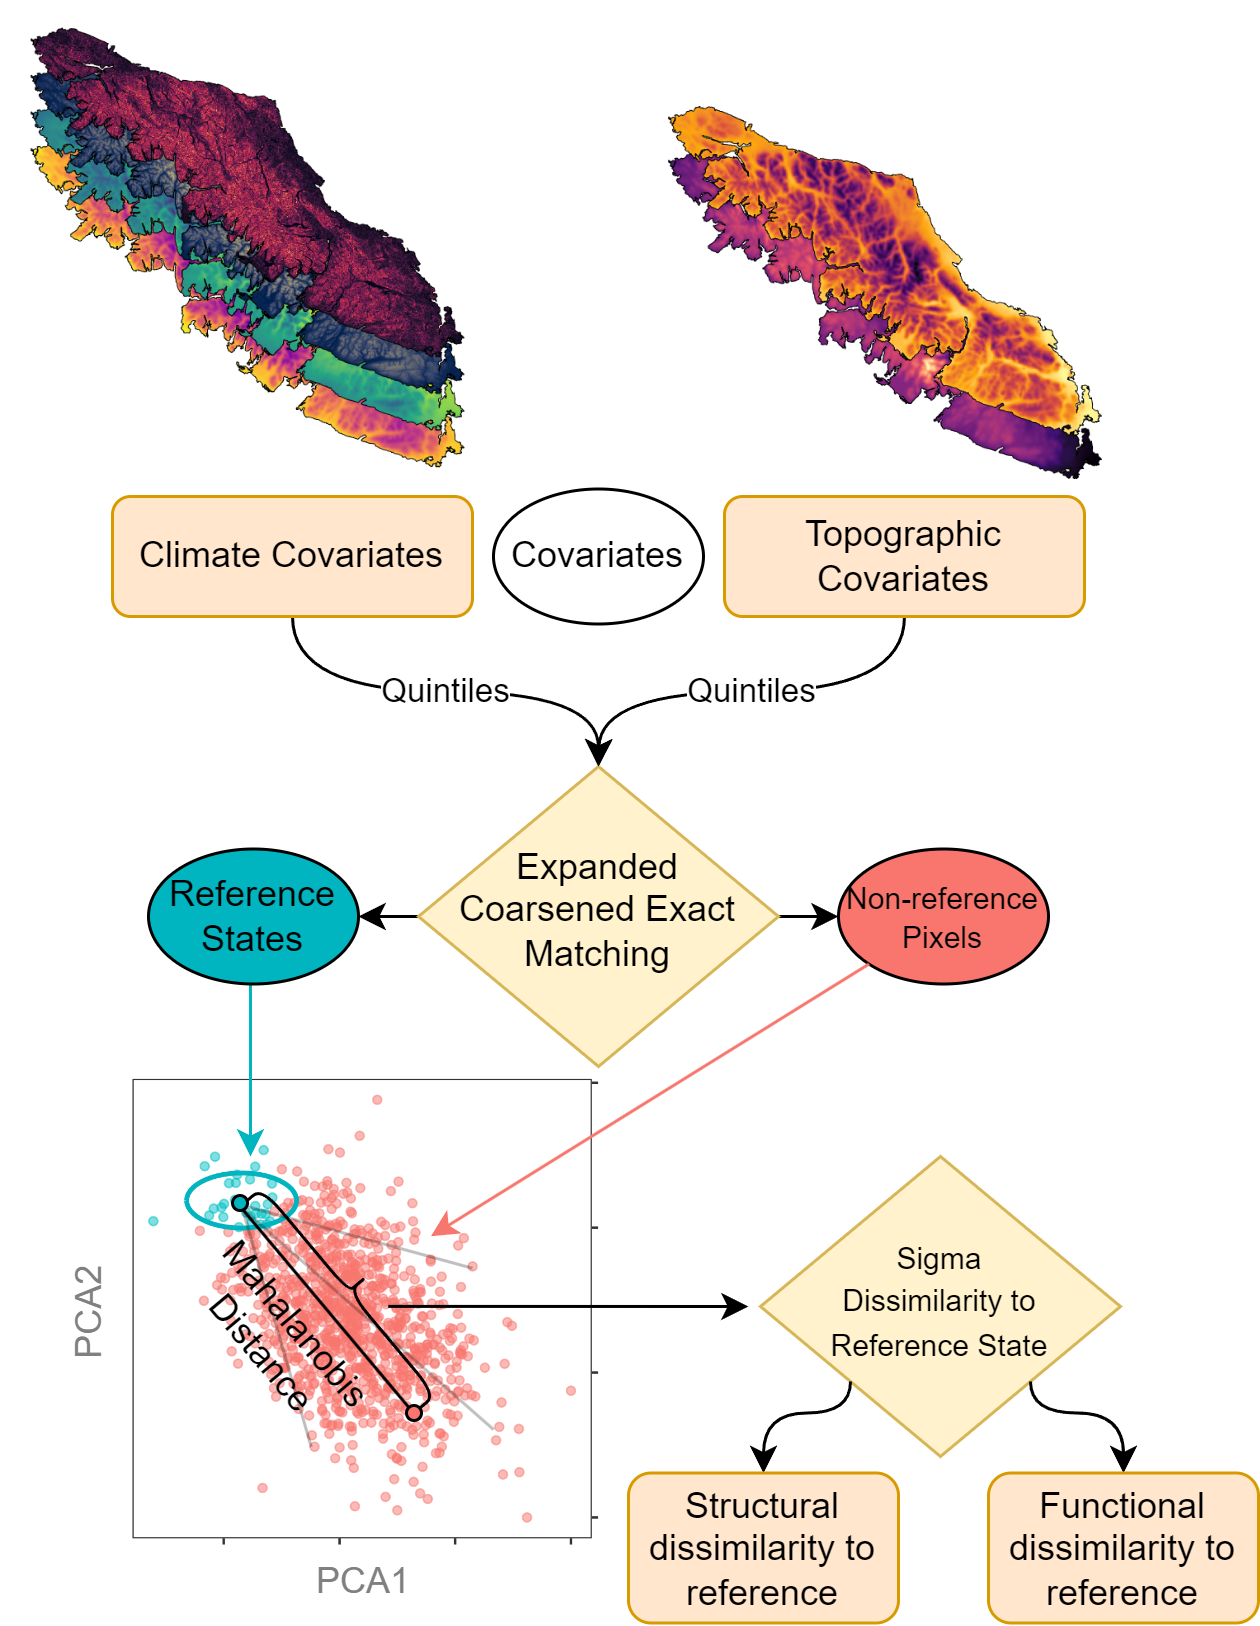
\includegraphics[width=4.05in,height=\textheight]{figures/flow.drawio.png}

}

\caption{\label{fig-flow}Conceptual flow diagram of the study.}

\end{figure}%

\subsection{Study Area}\label{sec-study}

We focus on the forested areas of Vancouver Island, British Columbia,
Canada (Figure~\ref{fig-study}). Vancouver Island has approximately
31,285 km\textsuperscript{2} of land area, of which 79.5\% is forested.
Climate is temperate maritime, with mild, wet winters, and cool, dry
summers. Vancouver Island is divided in four zones as defined by British
Columbia's biogeoclimatic ecosystem classification (BEC) framework
(Pojar et al., 1987), Coastal Western Hemlock, Mountain Hemlock, Coastal
Douglas-fir, and Coastal Mountain-heather Alpine, which are broadly
delineated based on climax vegetation species, soil, climate, and
elevation. We limit our analyses to Coastal Western Hemlock, Mountain
Hemlock, and Coastal Mountain-heather Alpine, as the Coastal Douglas-fir
ecosystem is not present within our reference state. The dominant tree
species on Vancouver Island are Douglas-fir (\emph{Pseudotsuga
menziesii}), western red cedar (\emph{Thuja plicata}), western hemlock
(\emph{Tsuga heterophylla}), yellow cedar (\emph{Chamaecyparis
nootkatensis}), and Sitka spruce (\emph{Picea sitchensis}) (Burns,
1990). Fires on Vancouver Island have historically been infrequent and
of low severity (Daniels and Gray, 2006). Forestry is an important
industry on Vancouver Island, with the majority of the land base being
managed for timber production under various tenures (Ministry of Water,
Land and Resource Stewardship (WLRS), 2023). These harvesting practices
have led to a need to protect remaining high-integrity forests, and
restore degraded forests.

\subsubsection{Reference State}\label{reference-state}

Strathcona Park was used as reference state to prioritize areas of
minimal human impact and ecological continuity, and in order to provide
a robust benchmark for assessing forest ecosystems in their natural
state. It was established in 1911, and is the oldest and largest
protected area in British Columbia, encompassing
2,480\textsuperscript{2} km, with approximately 80\% designated as
wilderness and Nature Conservancy Areas under the Park Act ({``Park
{Act},''} 1996). These designations have ensured the preservation of
natural ecological processes, leaving the park relatively free from
anthropogenic disturbances over more than a century, with the exception
of relatively small areas of concentrated impacts, such as Mount
Washington Alpine Resort for recreational skiing and Myra Falls Mine.
Strathcona Park includes three of the island's BEC zones, Coastal
Western Hemlock, Mountain Hemlock, and Coastal Mountain-heather Alpine.
Recreational activity such as skiing and hiking are permitted within
Strathcona Park, and there are small unprotected regions within the park
boundaries in which mining is permitted.

\phantomsection\label{cell-fig-study}
\begin{figure}[H]

\centering{

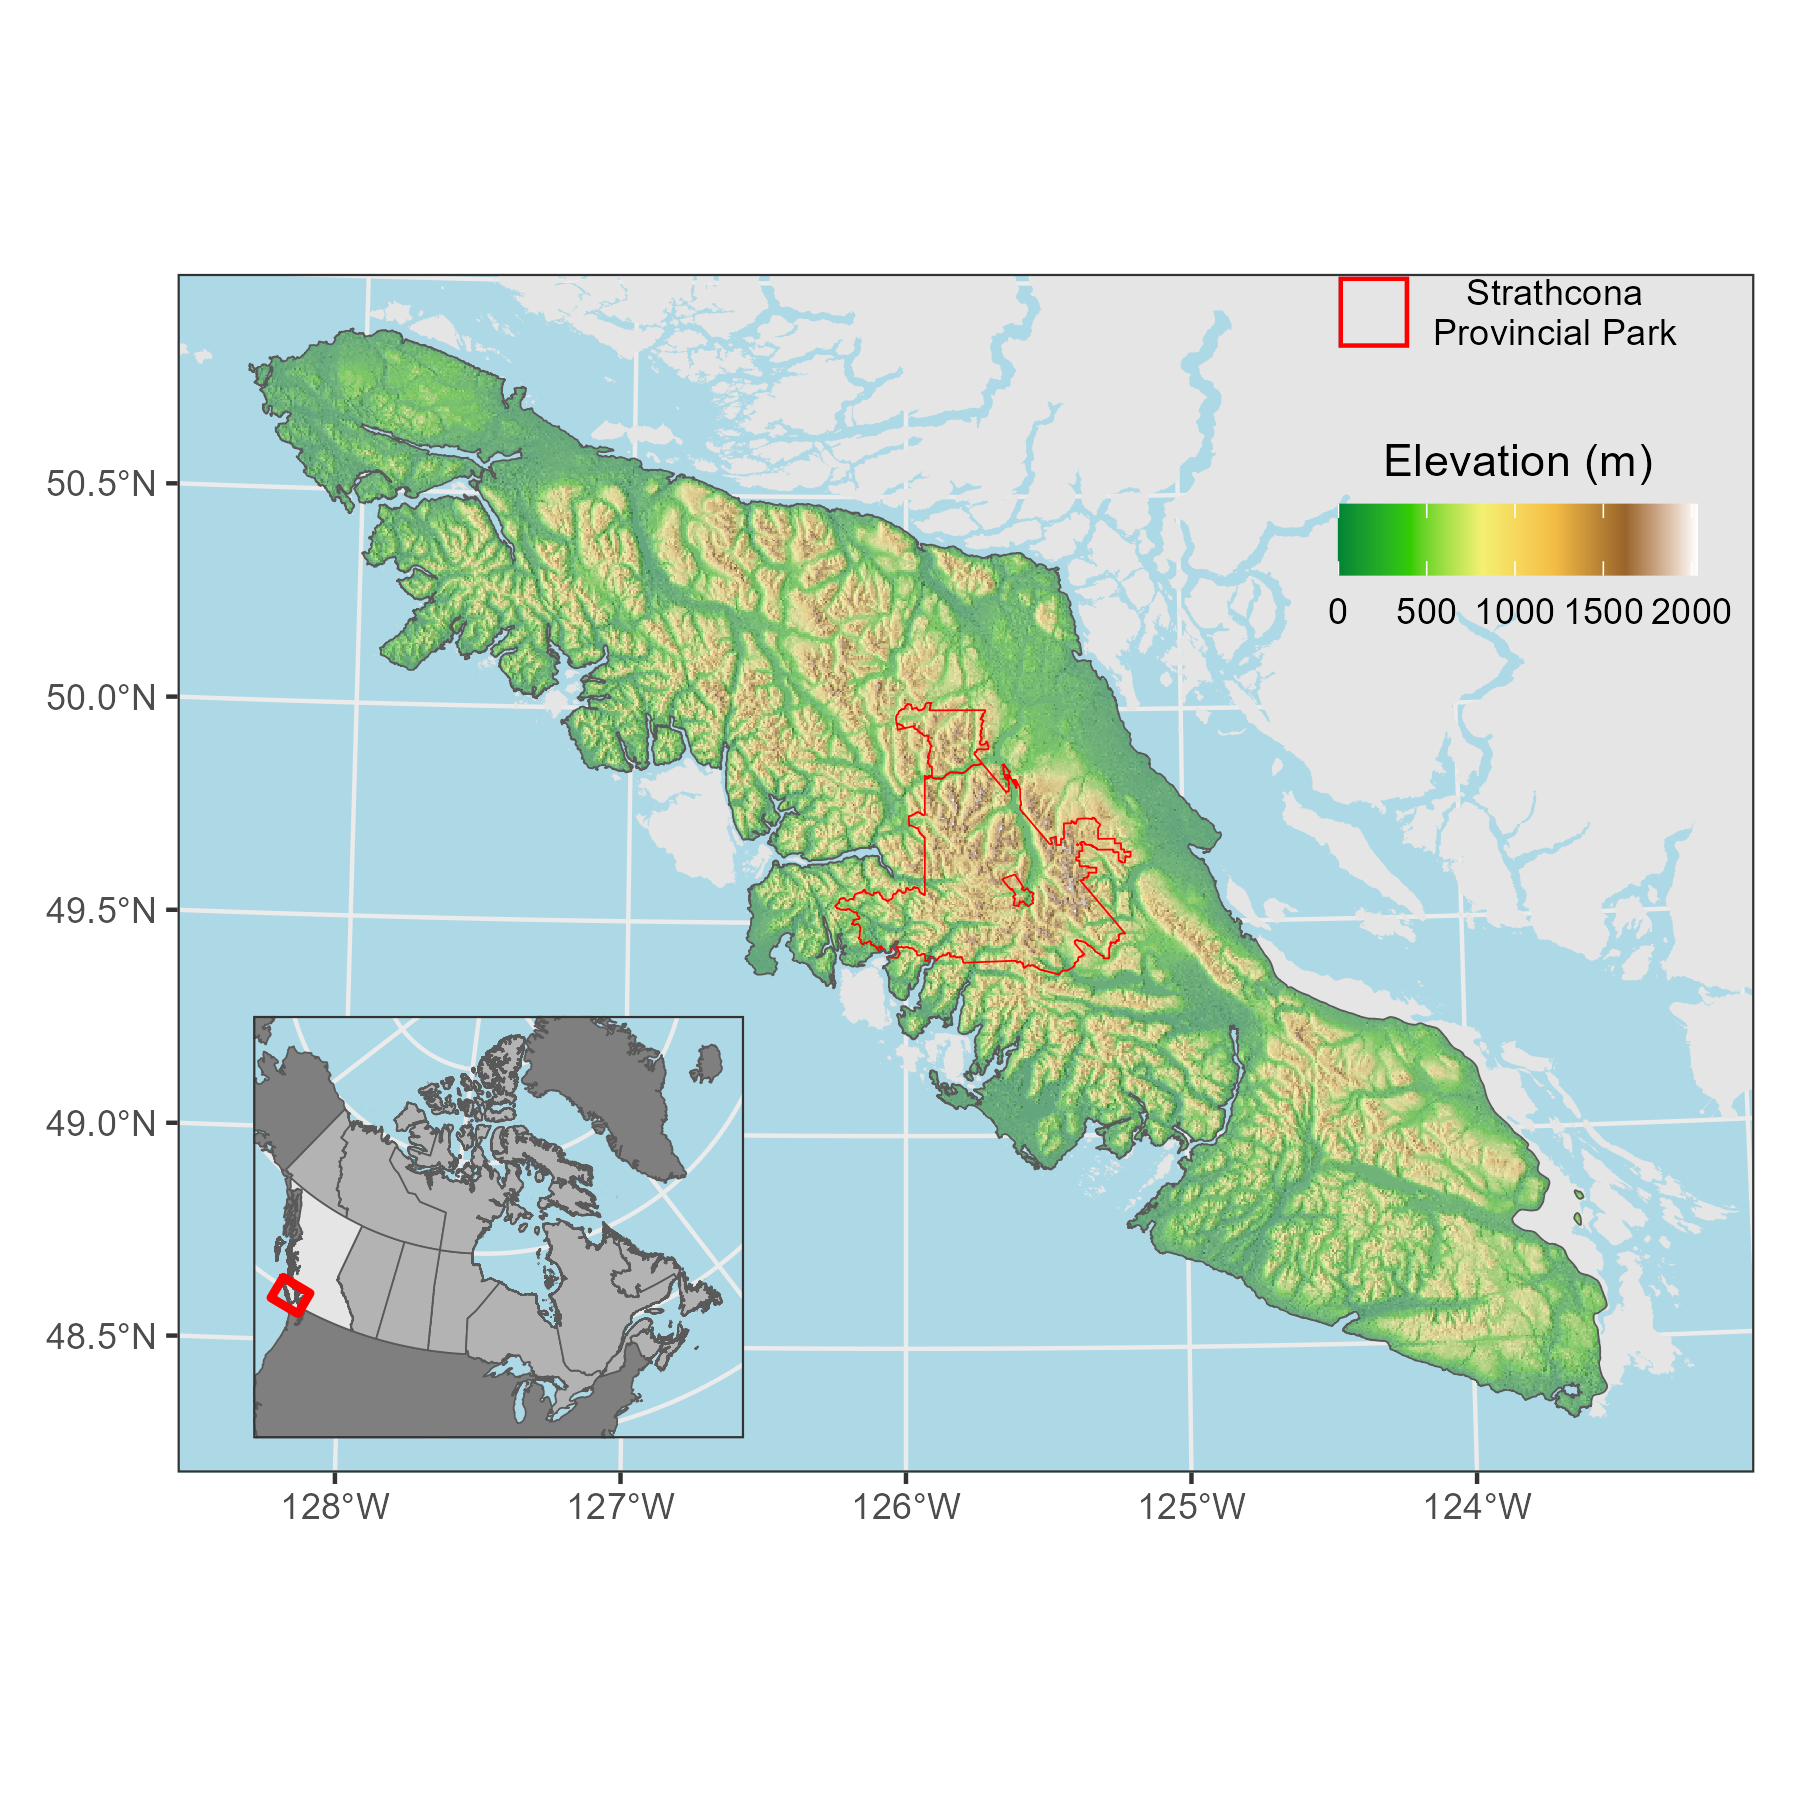
\includegraphics[width=6in,height=\textheight]{figures/study_area.png}

}

\caption{\label{fig-study}Study area on Vancouver Island, British
Columbia, Canada, including the location of Strathcona Park. In the
analysis we only include ecosystems found within Strathcona Park on the
primary land mass of Vancouver Island.}

\end{figure}%

\subsection{Data}\label{data}

\subsubsection{Forest Structure}\label{forest-structure}

Forest structure data were derived from the 30-m spatial resolution,
wall-to-wall layers generated by Matasci et al. (2018a; 2018b) for the
year 2015 using a random forest-kNN approach that imputed lidar-derived
forest structural attributes across Canada's forested ecosystems. We
chose the year 2015 as this data is freely available at
\url{https://opendata.nfis.org/mapserver/nfis-change_eng.html}. This
methodology used Landsat-derived best-available-pixel composites
representing growing season conditions (Hermosilla et al., 2016; White
et al., 2014), forest change information (Hermosilla et al., 2015a), and
topographic and positional information as predictors to impute forest
structural attributes by finding the most similar lidar plot within the
set of random forest trees. All forest structural attributes were
assigned at once, preserving the covariance in the response variables
and prohibiting overextrapolation. Accuracy metrics for the forest
structural attributes ranged from an RMSE of 29.7\% (structural
complexity) to 65.8\% (aboveground biomass) and R\textsuperscript{2}
values of 0.70 (aboveground biomass) to 0.13 (structural complexity)
(Matasci et al., 2018a; Matasci et al., 2018b).

\subsubsection{Forest Function}\label{forest-function}

To represent forest ecosystem function, we used the Dynamic Habitat
Indices (DHIs) dataset, which comprise a suite of intra-annual summaries
of energy availability (as represented by a vegetation index or estimate
of gross/net primary productivity) (Radeloff et al., 2019). The DHIs are
composed of the total available energy over the course of a year
(Cumulative DHI), the minimum amount of energy available over the course
of a year (Minimum DHI), and the variation in energy available over the
course of a year (Variation DHI). The DHIs were calculated at a 30-m
spatial resolution using Landsat data, following the methodology of
Razenkova (2023). The DHIs were computed on Google Earth Engine
(Gorelick et al., 2017) by creating a synthetic year of monthly NDVI
composites using all available Landsat imagery from 2011-2020 (centred
on 2015 to match the forest structural attribute data). We used the
Landsat QA band (Zhu and Woodcock, 2012) to filter pixels with clouds
and cloud shadows. Monthly NDVI values were calculated by taking the
median of each month's NDVI observations, ignoring the year the image
was acquired to increase the number of available images. The DHIs are
calculated as the sum (Cumulative DHI), minimum (Minimum DHI), and
coefficient of variation (Variation DHI) of these monthly observations.

\subsubsection{Anthropogenic Pressures}\label{anthropogenic-pressures}

We used the Canadian Human Footprint as developed by Hirsh-Pearson et
al. (2022) to inform on anthropogenic pressures on the environment. The
Canadian Human Footprint is an additive pressure map generated by
summing the 12 different anthropogenic pressures (built environments,
crop land, pasture land, population density, nighttime lights, railways,
roads, navigable waterways, dams and associated reservoirs, mining
activity, oil and gas, and forestry), which ranges from zero (lowest
pressure) to 55 (highest pressure) across Canada. This cumulative
dataset is also distributed with Canada-wide individual pressure values
(Hirsh-Pearson et al., 2022).

\subsubsection{Disturbance Mask}\label{disturbance-mask}

We use a forest disturbance mask to remove recently disturbed (since
1984) pixels from our reference states, developed by Hermosilla et al.
(2016), by using breakpoint analysis on normalized burn ratio values
derived from annual summer season growing condition best-available-pixel
composites (Hermosilla et al., 2015b; White et al., 2014). Detected
changes were attributed to a disturbance agent (harvest, wildfire,
non-stand replacing disturbances) using a random forest approach,
resulting in an overall accuracy of 92\% ± 1.4\% (Hermosilla et al.,
2016).

\subsubsection{Forest Cover Mask}\label{forest-cover-mask}

We used a land cover mask developed by Hermosilla et al. (2022; 2018) to
mask out non-forested areas from our analysis. This land cover mask was
developed by applying regional random forest models with an
inverse-distance-weighted approach and refined and calibrated predictor
data to identify 12 land cover classes, of which four are forested:
coniferous, broadleaf, mixed wood, and wetland-treed (Hermosilla et al.,
2022). Overall accuracy was 77.9\% ± 1.4\% across Canada (Hermosilla et
al., 2022).

\subsubsection{Topographic and climate
data}\label{topographic-and-climate-data}

We use a 30-m digital elevation model and derived slope dataset from the
Advanced Spaceborne Thermal Emission and Reflection Radiometer (ASTER)
Version 3 GDEM product (Abrams et al., 2020).

Climate variables: mean annual precipitation (MAP), mean annual
temperature (MAT), mean warmest month temperature (MWMT), and mean
coldest month temperature (MCMT) were calculated from 1990-2020 climate
normals using the ClimateNA software package at a 1 km spatial
resolution, and downsampled to 30-m using cubic spline resampling in the
\textbf{terra} (version 1.7-71) R package (Hijmans, 2024) in R (R Core
Team, 2024 version 4.4.1). A visualization of one of each input dataset
can be found in Figure~\ref{fig-data}.

\phantomsection\label{cell-fig-data}
\begin{figure}[H]

\centering{

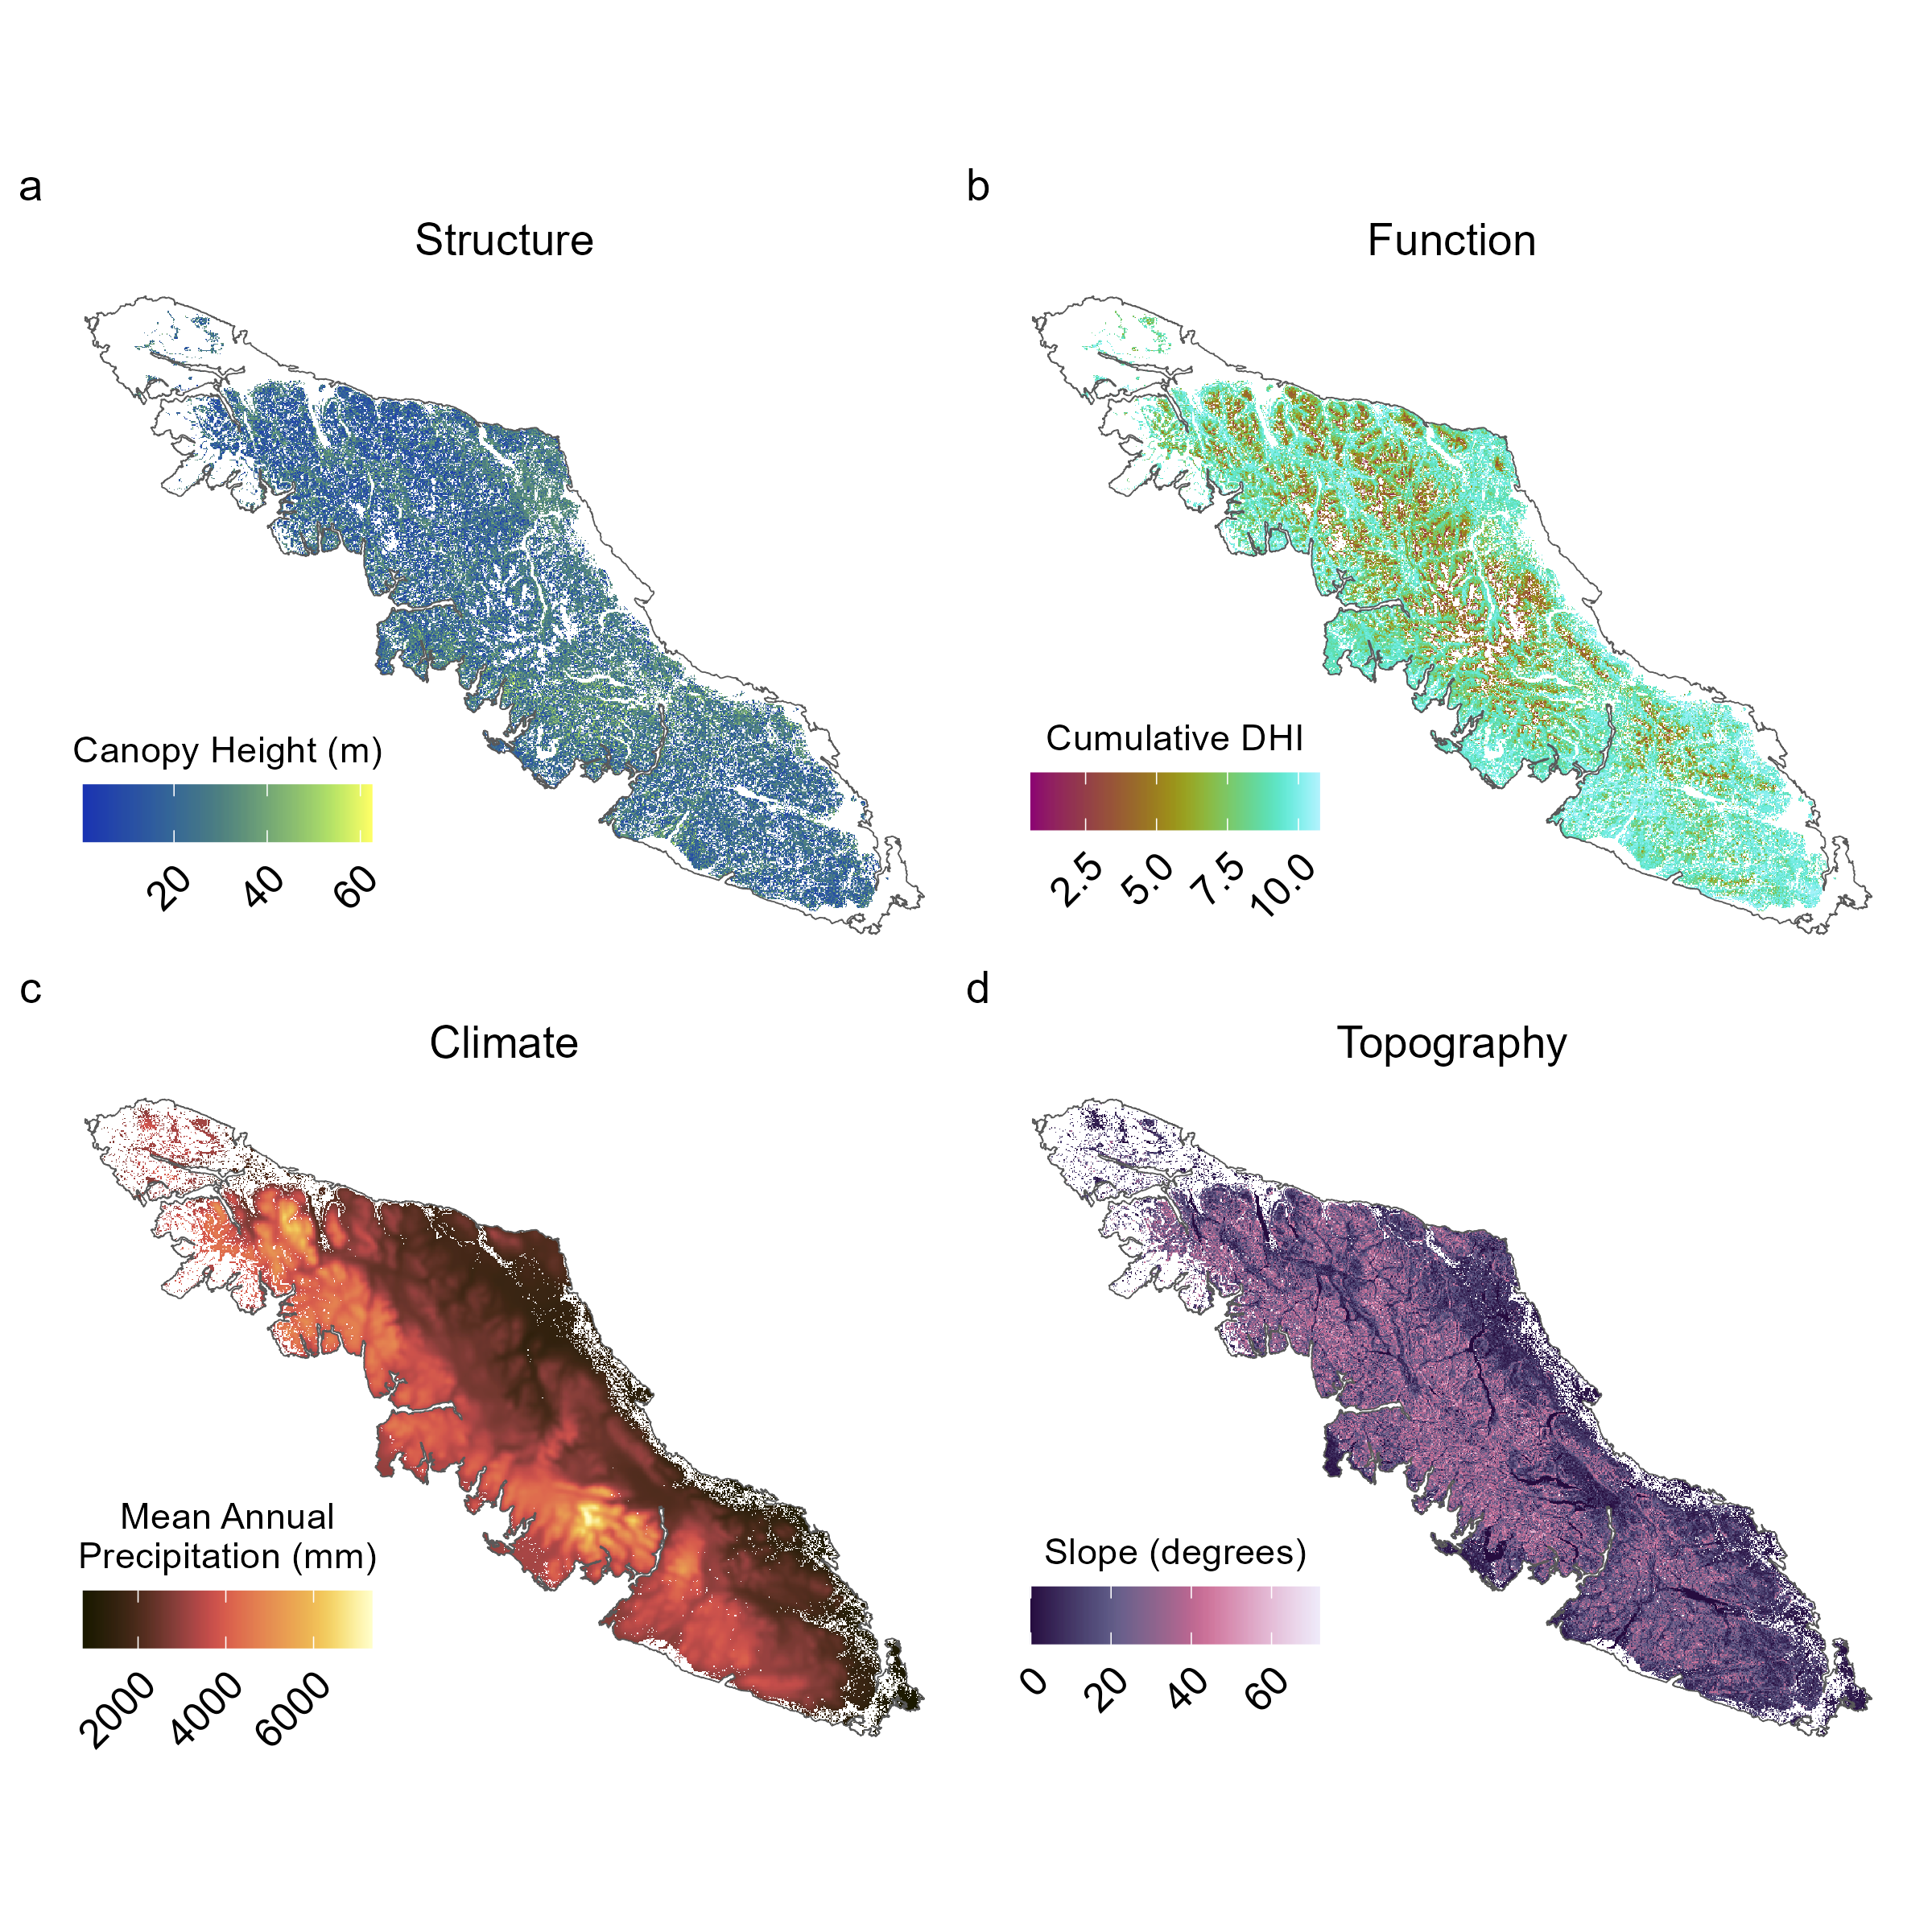
\includegraphics[width=8in,height=\textheight]{figures/data_figure.png}

}

\caption{\label{fig-data}Examples of each of the four major datasets
used in our study. Panels a and b show structure and function,
respectively, used for the calculation of sigma dissimilarity. Panels c
and d show climate and topography, respectively, used for the coarsened
exact matching procedure.}

\end{figure}%

\subsection{Metrics}\label{metrics}

We utilized four forest structural attributes generated by Matasci et
al. (2018a; 2018b): canopy height (95th percentile of elevation
returns), canopy cover (percentage of first returns above 2m),
structural complexity (coefficient of variation of elevation returns),
and aboveground biomass. Canopy height, canopy cover, structural
complexity are standardized lidar-derived metrics suitable for
biodiversity monitoring at the ecosystem scale (Valbuena et al., 2020).
The fourth attribute, aboveground biomass, represents the key ecosystem
service of carbon sequestration (Naidoo and Ricketts, 2006), and is
likely moderated by the three lidar-derived variables (Ali, 2019).

For the forest function metrics, we used the Cumulative and Variation
DHIs. We did not use the minimum DHI, which was consistently 0, due to
the presence of snow during winter in our study area. The DHIs have been
shown to be indicative of ecosystem functioning, as they represent
energy availability and seasonality (Berry et al., 2007), which is
correlated with biodiversity over a range of scales (Radeloff et al.,
2019; Razenkova et al., 2022), extents (Coops et al., 2019, 2009) and
taxa (Andrew et al., 2024; Coops et al., 2019).

\subsection{Calculating Ecological Dissimilarity}\label{sec-sim}

We calculated the sigma dissimilarity (Mahony et al., 2017) of forested
pixels across our study area using an expanded coarsened exact matching
(CEM) technique (Iacus et al., 2012) for each forest type: broadleaf,
coniferous, mixedwood, and wetland-treed (Hermosilla et al., 2022;
Hermosilla et al., 2018). The CEM technique creates comparable groups of
observations by first coarsening covariates into bins. In this study,
all six covariates---elevation, slope, mean annual precipitation (MAP),
mean annual temperature (MAT), mean coldest month temperature (MCMT),
and mean warmest month temperature (MWMT)---were coarsened into five
equally sized quintiles (bins). CEM then performs exact matching on
these bins, with each pixel matched to a climatically and
topographically similar group of pixels within the reference state
(Strathcona Park). We use the anthropogenic pressure layers to further
refine our reference state by excluding pixels with any amount of
anthropogenic pressure in Strathcona Park, and also removed pixels
disturbed since 1984 from the reference state. These matched groups are
referred to as strata. If insufficient reference state pixels were
identified within a stratum, we sampled up to 100 pixels from the
nearest neighbours across climate and topographic bins, minimizing the
nearest neighbour distance. Strata with average nearest neighbour
distances greater than or equal to two were excluded from the analysis
as they did not have an environmentally similar reference state to
compare to.

We then calculated the sigma dissimilarity metric to assess the
dissimilarity of all pixels---based on structural, functional, and
combined structural and functional attributes---relative to the
reference states. We first transformed the variables into principal
components, and calculated the euclidean distance from the reference
states mean centroid for all pixels, by stratum. This is also called the
Mahalanobis distance, and accounts for covariations in the data
(Mahalanobis, 1936). We then convert the Mahalanobis distance into sigma
dissimilarity by rescaling it into percentiles of the chi distribution
with one degree of freedom, accounting for the effect of dimensionality
in creating a multivariate dissimilarity metric (Mahony et al., 2017).
This metric serves as a proxy for ecological integrity, with higher
values indicating greater deviation from near-natural conditions
observed in the reference state.

\subsection{Impact of Anthropogenic Pressure on Ecological
Dissimilarity}\label{impact-of-anthropogenic-pressure-on-ecological-dissimilarity}

Here, we assessed the impact of the cumulative pressure map and four
individual pressures: population density, built environments, roads, and
forestry. We selected these four as other pressures (oil and gas;
railroads) are not present on Vancouver Island, while pasture land and
crop land do not coincide with currently forested areas. We reclassify
the overall Canadian Human Footprint (Hirsh-Pearson et al., 2022) and
individual pressures into categorical data following Hirsh-Pearson et
al. (2022) and Arias-Patino et al. (2024): a value of zero is considered
intact, zero to four has low anthropogenic pressure, four to eight has
medium anthropogenic pressure, and above eight has high anthropogenic
pressure.

To assess the cumulative impact of anthropogenic pressure on ecological
dissimilarity, we implemented stratified sampling on all suitable
stratum, sampling 100 pixels from each anthropogenic pressure class with
a minimum distance between samples of 1000 m. For our individual
pressures, we sampled an additional 100 pixels for each pressure class
with a minimum distance between samples of 1000 m. Sampling was
performed using the \textbf{sgsR} (version 1.4.5) R package (Goodbody et
al., 2023) with the Quiennec method. The Quiennec method ensures that
samples are drawn from regions surrounded by identical values, meaning
no edge pixels are selected (Queinnec et al., 2021). Geospatial data
processing was performed using the \textbf{terra} (version 1.7-78)
(Hijmans, 2024) and \textbf{sf} (version 1.0-16) (Pebesma, 2018) R
packages.

We used a one-way analysis of variance (ANOVA) with a critical p-value
of 0.05 to identify statistically significant differences in the mean
similarity values across cumulative anthropogenic pressure classes. We
accounted for family-wise error rate in our ANOVAs using the
Holm-Bonferroni method (Holm, 1979), only continuing the analysis for
similarity variables with significant ANOVAs at the adjusted critical
value. We used a Tukey HSD post-hoc test to identify which means are
different from the control group (intact pixels), which also controls
for the family-wise error rate.

The difference in means for each anthropogenic pressure of interest
(roads, population density, forestry, and built environment) were
identified following the same protocol. We compared each pressure to the
same `no pressure' values sampled in the cumulative pressure analysis.
All statistical analysis were conducted using the \textbf{rstatix}
(version 0.7.2) R package (Kassambara, 2023).

\section{Results}\label{results}

We generated maps of sigma dissimilarity for ecosystem structure,
function, and combined structure and function over the study area in
Vancouver Island as a measure of ecological integrity
(Figure~\ref{fig-regional}). Three representative examples to display
the impact of anthropogenic pressures on ecosystem similarity are shown:
a region near Lake Cowichan where harvesting is a common pressure
(Figure~\ref{fig-regional} A), a protected area (Elk Falls Provincial
Park) near Campbell River with high population density
(Figure~\ref{fig-regional} B), and a region with lower anthropogenic
pressures (Figure~\ref{fig-regional} C). Functional dissimilarity shows
higher variation across all three sites than functional or combined
structural and functional dissimilarity. The protected region near
Campbell River (Figure~\ref{fig-regional} B) has lower dissimilarity
metrics for all three metrics.

\phantomsection\label{cell-fig-regional}
\begin{figure}[H]

\centering{

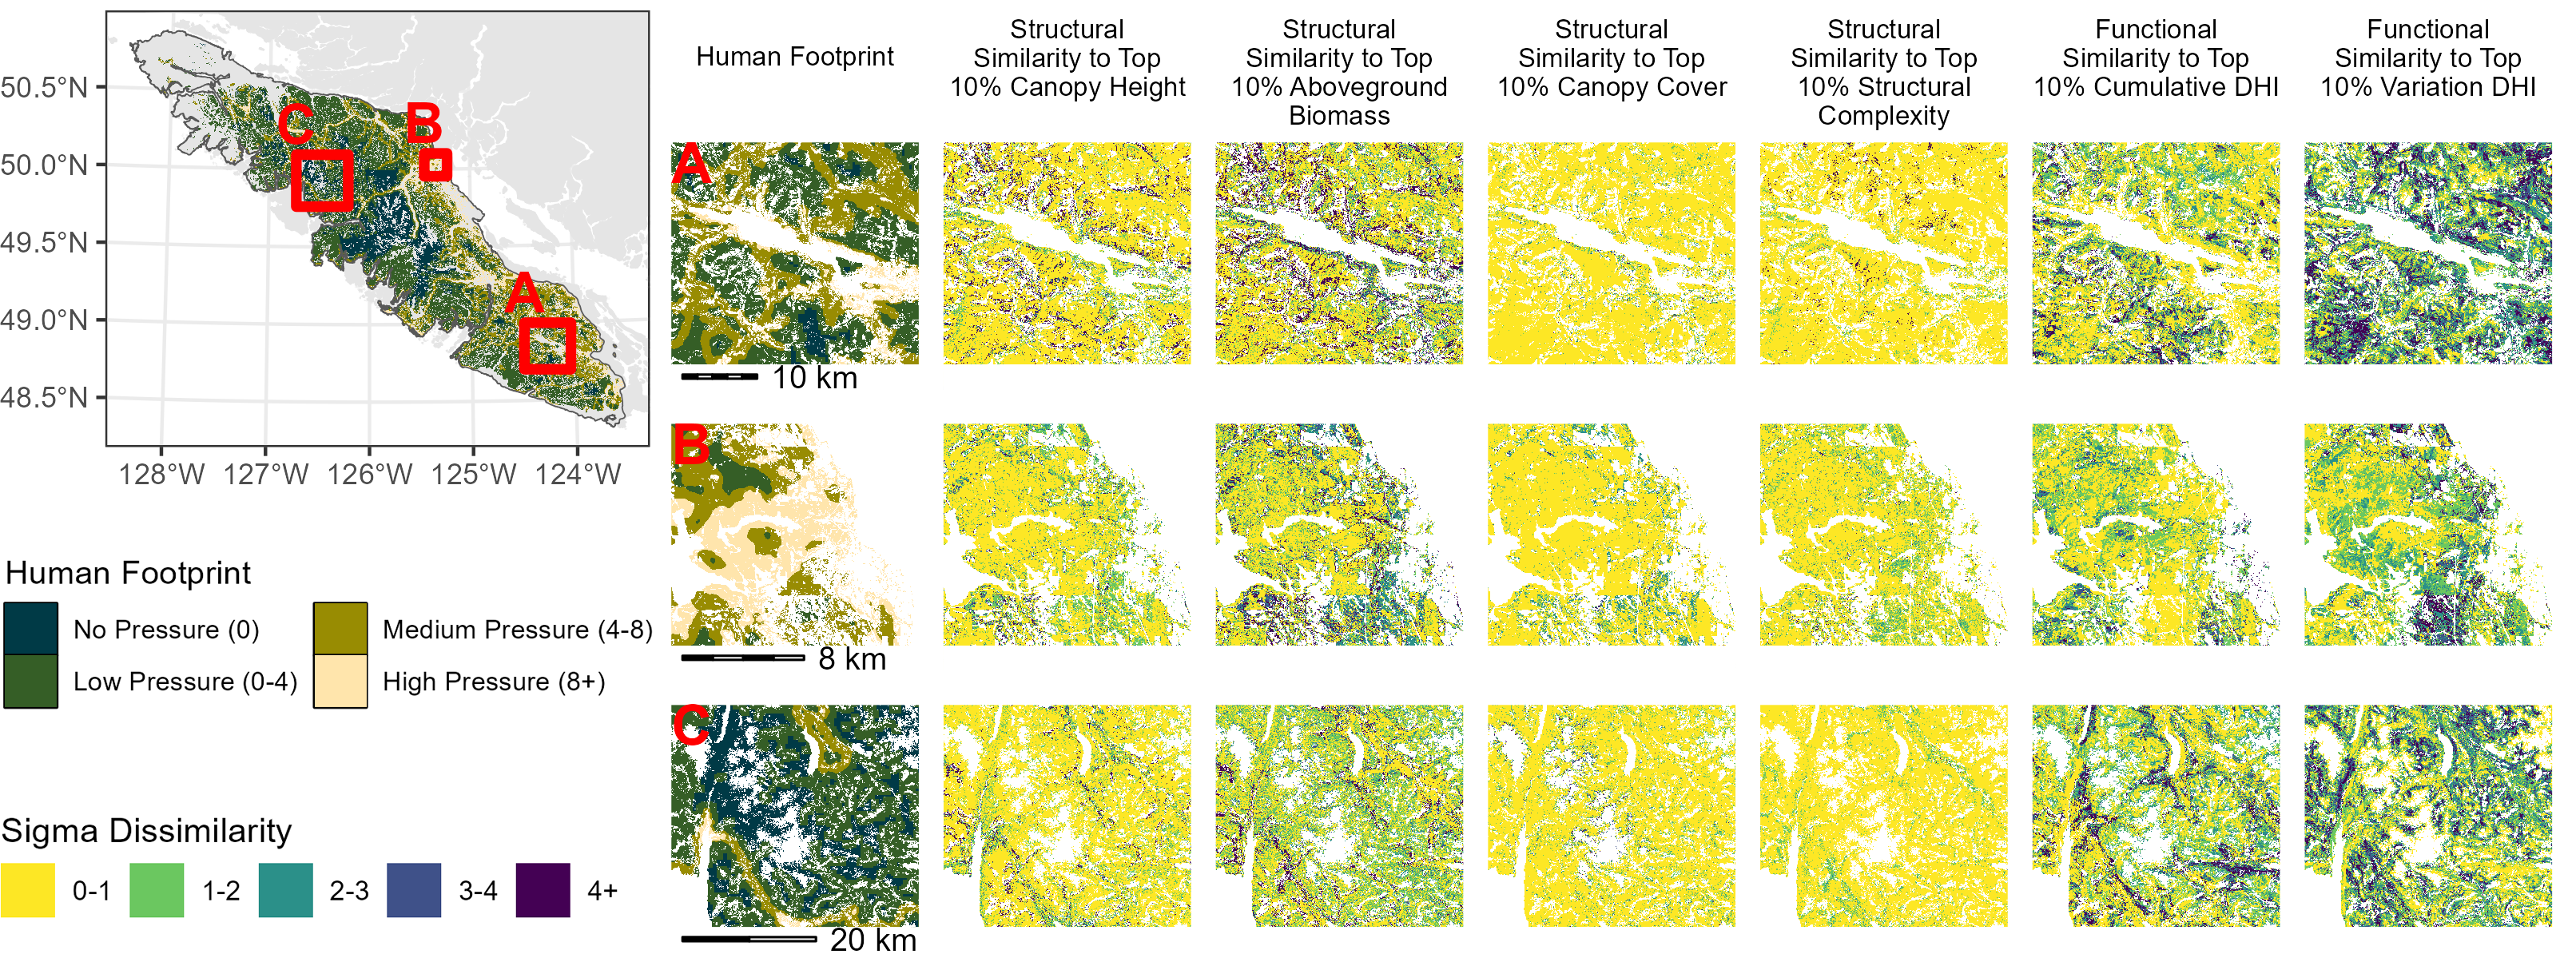
\includegraphics[width=10in,height=\textheight]{figures/multi_panel_inset_wide_PS.png}

}

\caption{\label{fig-regional}Regional details of the human footprint and
sigma dissimilarity across the sites on Vancouver Island. Note that
non-forested pixels and forested pixels without suitable matches (nn
\textgreater{} 2) are not shown. Subset A show Cowichan Lake, a heavily
harvested region. Subset B shows Elk Falls Provincial Park, just outside
Campbell River, a region with high population density. Subset C shows a
region with generally low anthropogenic pressure.}

\end{figure}%

Results on the influence of the cumulative human footprint on ecological
dissimilarity indicate that mean structural (ANOVA; p = 0.014) and
combined structural and functional (ANOVA; p = 0.006) dissimilarity was
significantly different under varying anthropogenic pressures
(Figure~\ref{fig-boxplot-overall}). We found no evidence that the
functional dissimilarity metric significantly varied with anthropogenic
pressures. The Tukey HSD test revealed that high levels of anthropogenic
pressures significantly influenced dissimilarity to the structural
reference state, increasing from 0.11 to 0.24 (ANOVA; p \textless{}
0.01), and to the combined structural and functional reference state,
increasing from 0.02 to 0.07 (ANOVA; p \textless{} 0.05). Medium and low
levels of anthropogenic pressures did not significantly influence any
dissimilarity

\phantomsection\label{cell-fig-boxplot-overall}
\begin{figure}[H]

\centering{

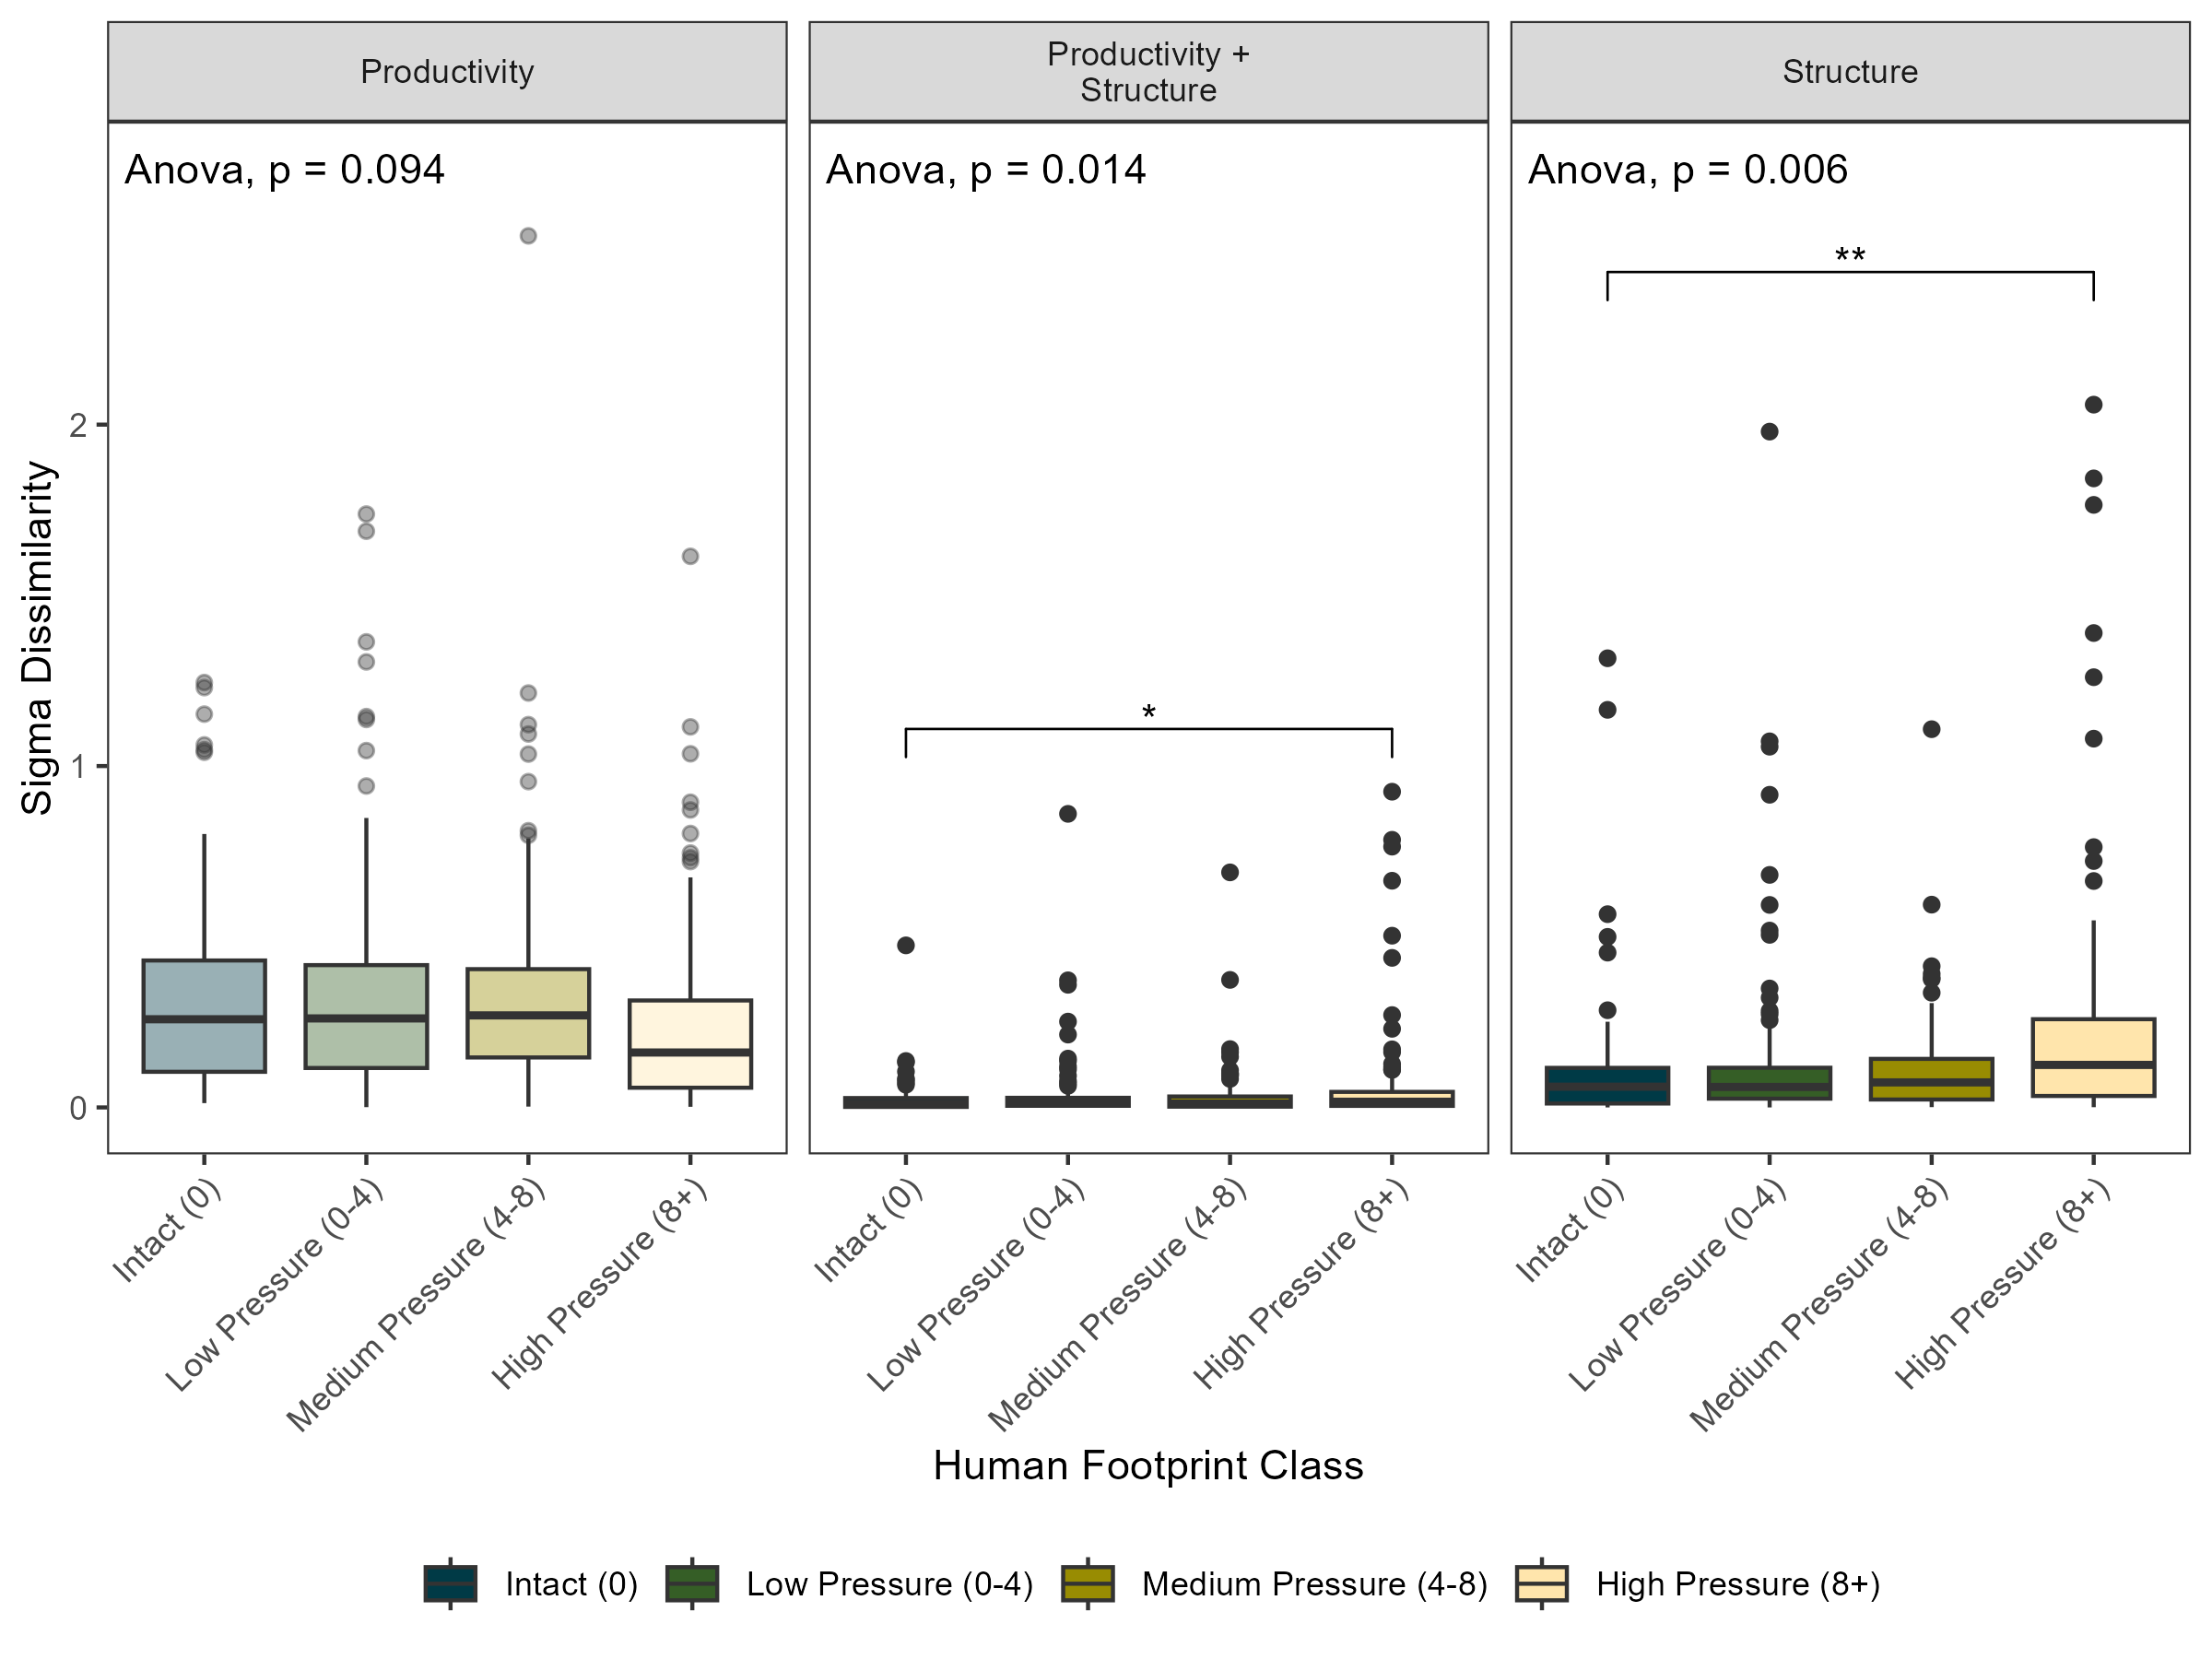
\includegraphics[width=8in,height=\textheight]{figures/mahal_boxplot_sig.png}

}

\caption{\label{fig-boxplot-overall}Boxplots of sigma similarity to the
reference state in Strathcona Park by cumulative human footprint
category. ANOVA p-values corrected using the Holm-Bonferroni method. *
indicates a Tukey HSD p-value \textless{} 0.05. ** indicates a Tukey HSD
p-value \textless{} 0.01.}

\end{figure}%

The assessment of the impact of individual pressures on ecological
dissimilarity to the reference state
(Figure~\ref{fig-boxplot-individual}) indicated that functional
dissimilarity was not significantly influenced by any anthropogenic
pressures, and that roads did not influence any type of ecological
dissimilarity (ANOVAs; all p \textgreater{} 0.05). Population density,
forestry and harvesting, and built environments did significantly
increase both structural and combined structural and functional
dissimilarity (ANOVAs; all p \textless{} 0.01). Only the highest levels
of pressures for each anthropogenic pressure category significantly
influenced ecological dissimilarity (ANOVAs; all p \textless{} 0.01).

\phantomsection\label{cell-fig-boxplot-individual}
\begin{figure}[H]

\centering{

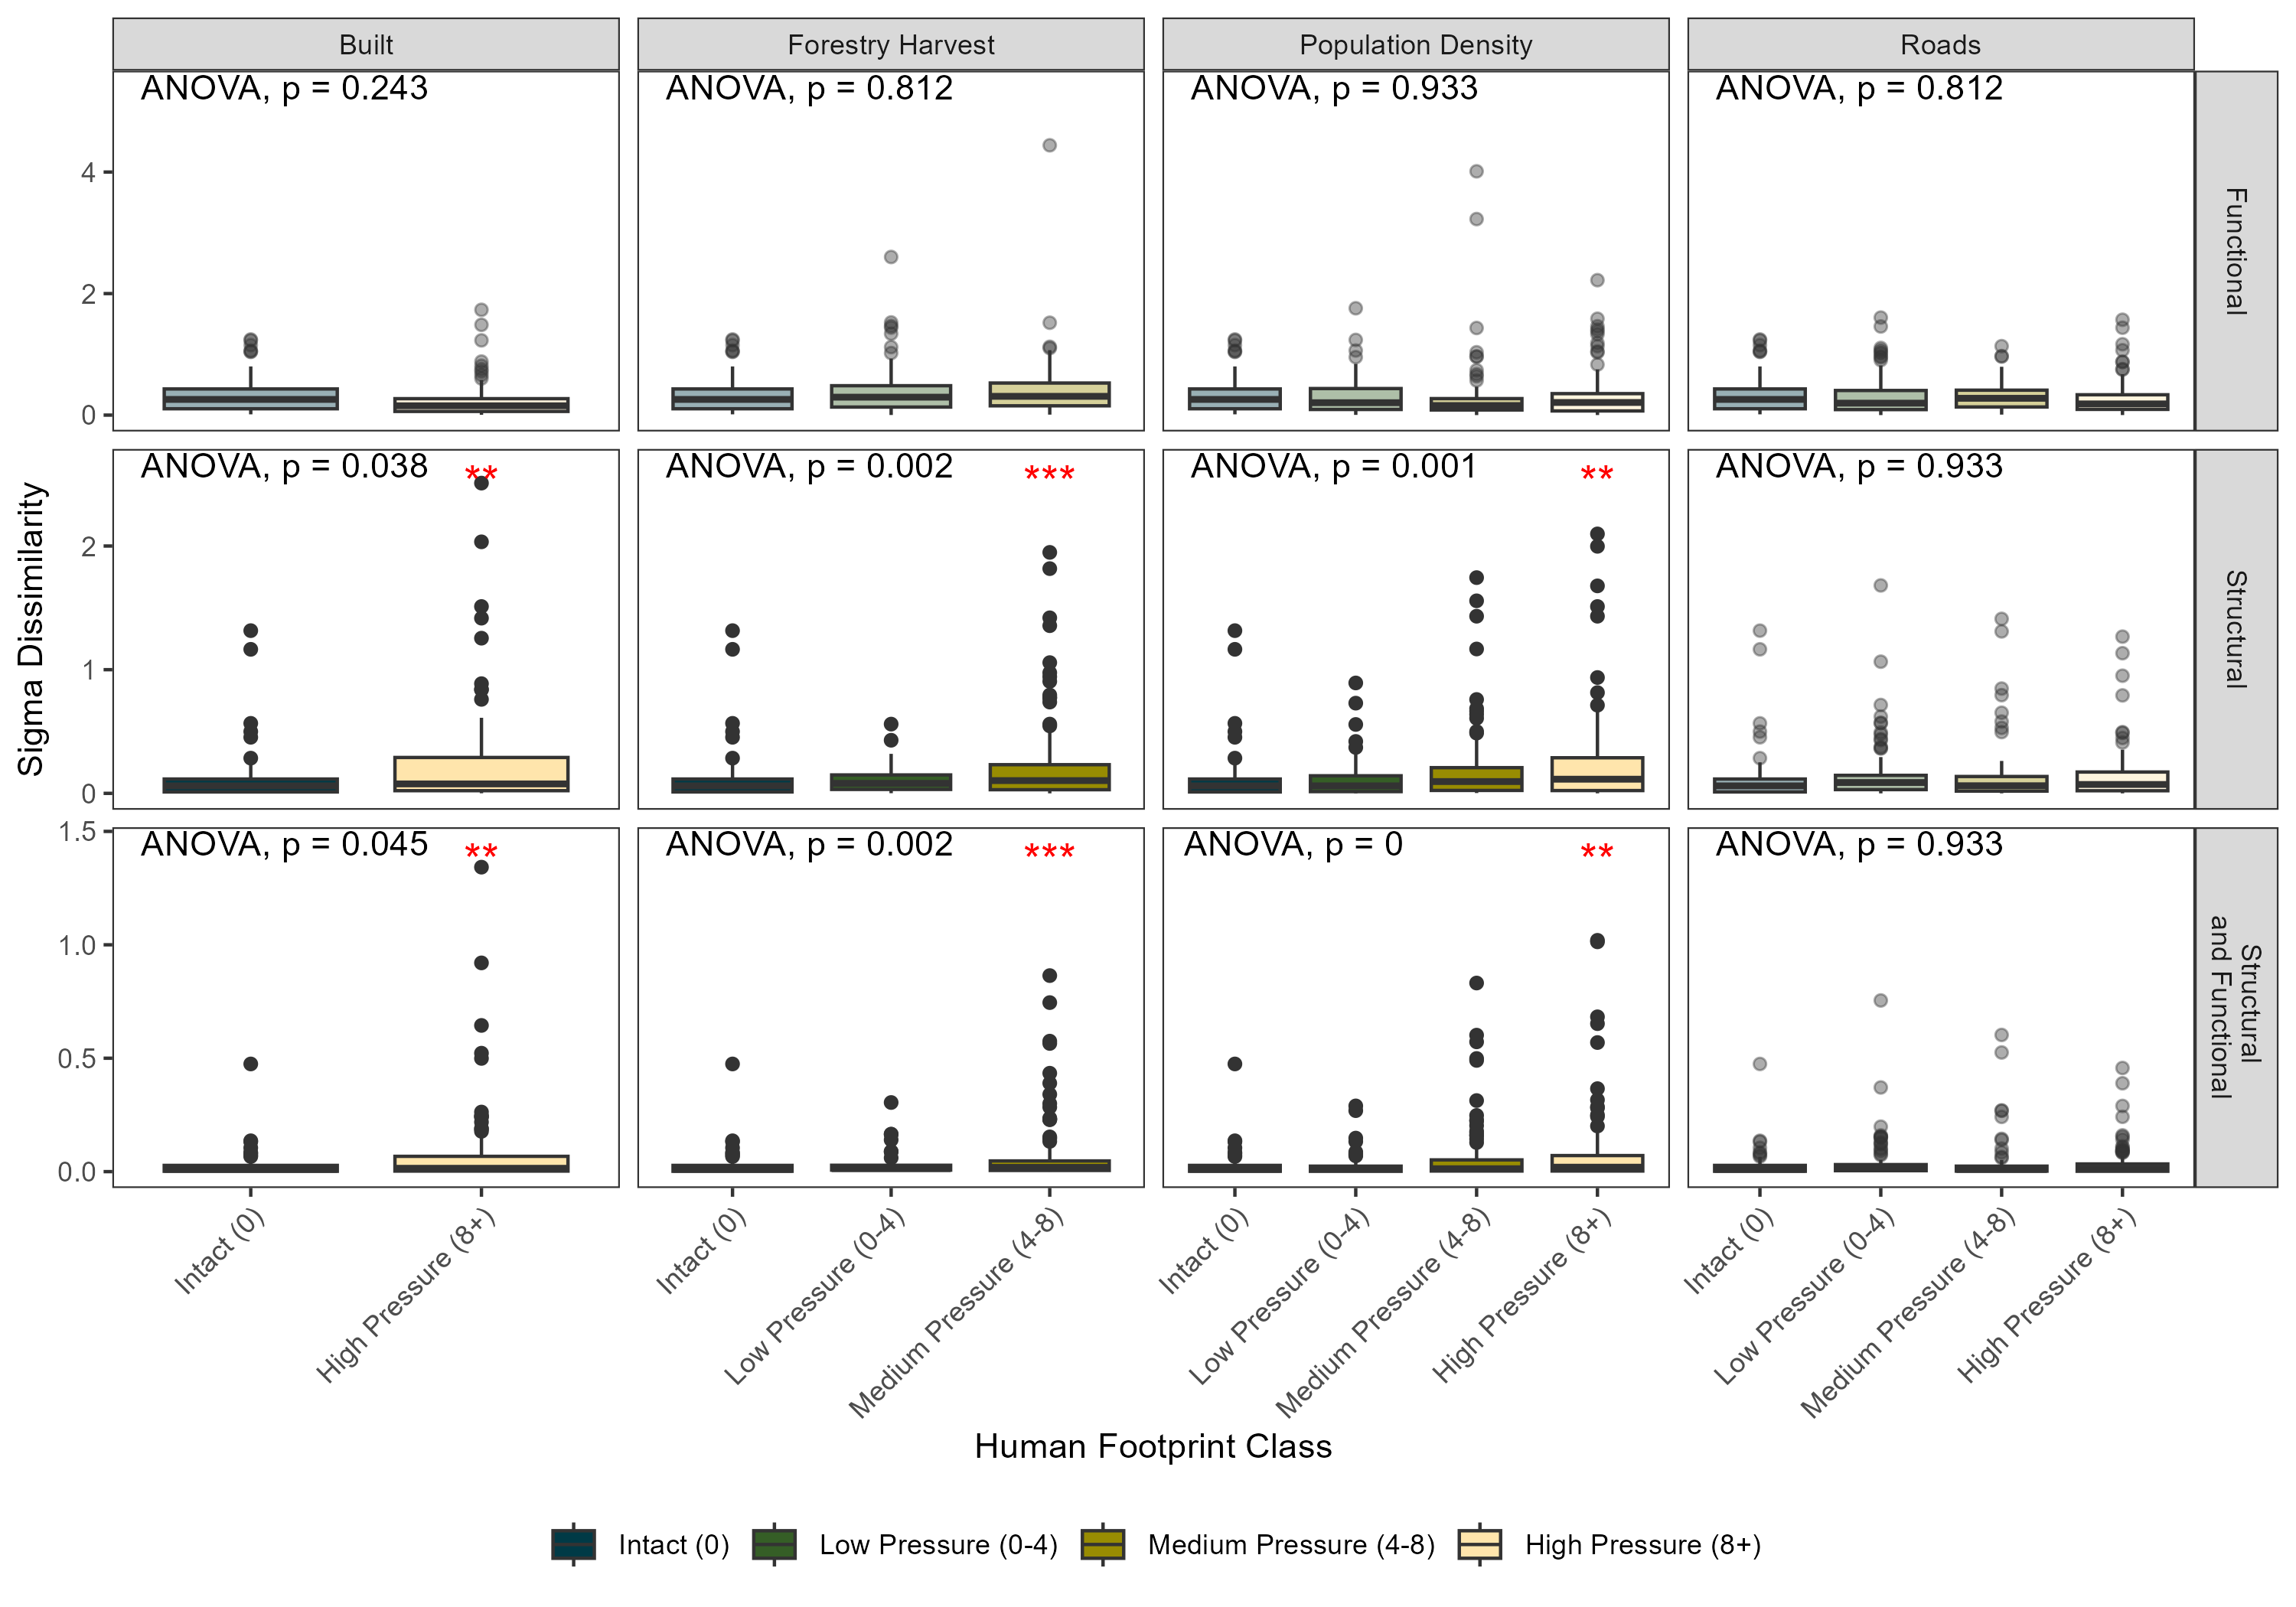
\includegraphics[width=10in,height=\textheight]{figures/indiv_boxplots.png}

}

\caption{\label{fig-boxplot-individual}Boxplots of sigma similarity to
the reference state in Strathcona Park by individual anthropogenic
pressures. ANOVA p-values corrected using the Holm-Bonferroni method. **
indicates a Tukey HSD p-value \textless{} 0.01. *** indicates a Tukey
HSD p-value \textless{} 0.001.}

\end{figure}%

\section{Discussion}\label{discussion}

There is a growing need to move beyond area-based approaches to
conservation. The GBF proposes to protected 30\% of all ecosystems by
2030, emphasizing the preservation of high-integrity ecosystems
(Convention on Biological Diversity, 2023; Ferrier et al., 2024).
However, data and approaches for delineating high-integrity ecosystems
are currently lacking. In this study, we developed a novel, data-driven
framework to assess ecological integrity in forested landscapes, using
coarsened exact matching (Iacus et al., 2012) to establish robust
reference states and sigma dissimilarity metrics (Mahony et al., 2017)
to quantify structural and functional deviations from these
high-integrity conditions. The approach was demonstrated using forested
areas on Vancouver Island, with Strathcona Park serving as the reference
state due to its environmental similarity to the study area. Results
indicate that high levels of anthropogenic pressure significantly
increase structural and combined structural and functional
dissimilarity, highlighting a reduction in ecological integrity
(Figure~\ref{fig-boxplot-overall}). In contrast, functional
dissimilarity remained unaffected by anthropogenic pressures,
potentially indicating a decoupling between forest structure and annual
energy availability (Muise et al., 2024), even under varying levels of
anthropogenic pressure. Our results provide a scalable method for
mapping forest ecological integrity, offering valuable insights for
conservation planning, protected area management, and impact assessments
beyond the study area.

\subsection{Strengths and Limitations for a Data-Driven Approach to
Assessing Forest
Integrity}\label{strengths-and-limitations-for-a-data-driven-approach-to-assessing-forest-integrity}

Our methodology offers several advantages in assessing ecological
integrity at regional and national scales, including a lack of
information on high quality reference states, the ability to incorporate
and compare across multiple indicators of ecological integrity, and the
transferability of the methods. By leveraging a robust, data-driven
reference state derived from a large, long-established protected area,
we ensure that comparisons are made against ecologically intact
ecosystems that are both attainable and environmentally consistent with
areas being evaluated (McNellie et al., 2020). The use of the sigma
dissimilarity metric allows for a more nuanced evaluation of ecological
integrity by accounting for covariations in the data and adapting to
varying dimensionality in input datasets (Mahony et al., 2017), reducing
biases associated with univariate assessments. Additionally, our
approach enhances environmental consistency by employing an expanded
coarsened exact matching technique (Iacus et al., 2012), which preserves
environmental comparability between reference states and assessed
forests. These methodological advancements improve the transferability
of ecological integrity assessments across different forested
ecosystems, providing a scalable and adaptable framework for
conservation planning.

Our structural dissimilarity metric offers a flexible, data-driven
alternative to traditional forest integrity assessments, enhancing its
applicability across diverse ecosystems. Unlike threshold-based
approaches, which often require predefined benchmarks for structural
integrity (Hansen et al., 2019), our method uses sigma dissimilarity to
the reference state to quantify ecological integrity in a multivariate
and context-specific manner. This adaptability makes our framework more
transferable to different forested ecosystems, as it does not assume a
fixed structural composition but instead evaluates integrity based on
the relative similarity to a high-integrity reference state, following
the definition of ecological integrity (Hansen et al., 2021). By
integrating both structural and functional dimensions, our methodology
allows for a broader applicability beyond temperate or tropical forests,
making it a valuable tool for conservation planning across diverse
forested regions.

Often, impact evaluation methods applied to conservation systems seek to
determine the system wide differences between protected and unprotected
areas, which are often reported as a single value (Ferraro, 2009;
Geldmann et al., 2019). Here, by integrating matching techniques with a
multidimensional dissimilarity metric, we can generate
spatially-explicit maps of ecological dissimilarity, providing insight
beyond the overall difference between protected and unprotected areas.
This gives a more comprehensive understanding of protected area
effectiveness, and can allow for improved prioritization of conservation
resources and allows for the analysis of ecological integrity with other
datasets, such as the human footprint (Arias-Patino et al., 2024;
Hirsh-Pearson et al., 2022).

Our methodology provides a versatile framework for conservation and
habitat assessments, with applications extending beyond Vancouver
Island's forested ecosystems. For example, this framework can be applied
to identify high-quality habitat for species with specific structural
requirements, such as the marbled murrelet (\emph{Brachyramphus
marmoratus}), which relies on old-growth forests with tall, complex
canopies for nesting (Cosgrove et al., 2024). Additionally, the ability
to quantify ecological dissimilarity across landscapes enables its use
in protected area prioritization, landscape connectivity analysis, and
ecological restoration planning. As global conservation efforts, such as
the 30x30 goal, emphasize the need for protecting high-integrity
ecosystems (Convention on Biological Diversity, 2023), our approach
offers a scalable and transferable tool for identifying and managing
critical conservation areas.

A key challenge in applying our methodology lies in selecting an
appropriate reference state, which is integral for accurately measuring
ecological integrity. The selection of an appropriate reference state is
critical, as the ecological integrity of assessed forests is measured
relative to this benchmark (McNellie et al., 2020). While our use of a
large, long-established protected area ensures minimal anthropogenic
influence, differences in environmental conditions between the reference
and assessed areas could introduce variability, especially in cases
where no perfect match is found. We could potentially include additional
areas as reference states to reduce the number of imperfect or
unavailable matches, however, nearly all of the protected areas on
Vancouver Island do not meet our large and long-established criterion.
Thus, there are tradeoffs to be considered when expanding the reference
state to additional newer or smaller parks.

\subsection{Ecological Integrity and Anthropogenic Pressures on
Vancouver
Island}\label{ecological-integrity-and-anthropogenic-pressures-on-vancouver-island}

Our results indicate that high levels of cumulative anthropogenic
pressure led to increased structural dissimilarity, demonstrating a
small but significant decline in forest ecological integrity
(Figure~\ref{fig-boxplot-overall}). This aligns with previous studies
that have identified structural degradation under anthropogenic
influence (Bourgoin et al., 2024; Li et al., 2023), though our approach
extends these findings by applying a multivariate dissimilarity metric
rather than relying on singular structural indicators such as canopy
height or biomass. The observed structural dissimilarity suggests that
human activities are altering forest structure, reducing its resemblance
to high-integrity reference states. These results highlight the need for
conservation strategies that mitigate structural degradation,
particularly in regions experiencing increasing human pressures.

Examining the impact of individual anthropogenic pressures on forest
structure revealed varying effects, with most pressures contributing to
increased structural dissimilarity
(Figure~\ref{fig-boxplot-individual}). However, roads did not
significantly impact structural dissimilarity, contrasting with other
pressures such as built environments, harvesting, and population
density, which all led to measurable increases in structural
dissimilarity. These results suggests that while roads can fragment
landscapes and alter connectivity, their direct influence on stand-level
forest structure may be less pronounced compared to land-uses that
actively modify vegetation composition and density (Bourgoin et al.,
2024; Wulder et al., 2011). Our findings emphasize the importance of
considering individual pressure types rather than relying solely on
cumulative impact metrics, as different pressures may drive ecological
degradation through distinct mechanisms. These individual component
results also contribute to discussions around anthropogenic pressure
mapping methods, as there is little information on the mechanistic
interactions between anthropogenic pressures (Arias-Patino et al.,
2024).

In contrast to structural dissimilarity, functional dissimilarity
exhibited stronger spatial variation (Figure~\ref{fig-regional}) but was
not significantly influenced by cumulative or individual anthropogenic
pressures (Figure~\ref{fig-boxplot-overall} ;
Figure~\ref{fig-boxplot-individual}). This suggests that functional
attributes of forests, such as productivity and seasonal dynamics, may
be more resilient to direct human pressures than structural
characteristics. While prior research has linked anthropogenic forest
degradation to changes in canopy function (Bourgoin et al., 2024), our
findings indicate that in temperate ecosystems with consistently high
canopy cover, such as Vancouver Island, functional metrics may not be
strongly linked to anthropogenic pressures. These results highlight the
complexity of ecosystem functioning and suggest that factors beyond
anthropogenic pressure, such as climate variability and natural
disturbance regimes, may play a dominant role in shaping functional
integrity.

Several factors may explain the lack of a significant anthropogenic
influence on functional dissimilarity. NDVI-based functional metrics,
such as the DHIs, are known to saturate in forests with high canopy
cover and leaf area index (Huete et al., 2002), which are prevalent in
our study area (Muise et al., 2024). Additionally, Vancouver Island's
temperate climate and dominance of coniferous forests may result in
relatively stable seasonal energy availability compared to ecosystems
with stronger seasonality, such as tropical or deciduous forests. The
low functional response to anthropogenic pressures observed in our study
suggests that alternative functional indicators, such as phenospectral
metrics (Osei Darko et al., 2024) or multi-spectral indices beyond NDVI,
may be needed to better capture human-induced functional changes in
forested landscapes. Future research should explore alternative
functional metrics that are less prone to saturation, particularly in
ecosystems with dense, evergreen canopies like those on Vancouver
Island.

\section{Conclusion}\label{conclusion}

As the international community moves toward the goal of protecting 30\%
of high-integrity ecosystems by 2030, it is critical to identify the
location of such ecosystems. However, identifying high-integrity forests
at the national or regional scales is difficult due to a lack of
comprehensive spatial data on high-integrity ecosystems and varying
definitions of what constitutes a high-integrity forest. In this study,
we propose a novel, data-driven framework to assess ecological integrity
in forested ecosystems. The methodology integrates a robust technique
for generating suitable reference states through the use of a large,
long-term protected area, and by excluding any pressures and
disturbances. Ecological integrity is estimated as dissimilarity to the
reference state by using the sigma dissimilarity metric, which accounts
for covariations in the data and varying dimensionality in input
datasets. We demonstrate our methodology on forested areas of Vancouver
Island which are environmentally similar to the reference state,
Strathcona Park. Furthermore, we assess the impact of anthropogenic
pressures on our metric, revealing that high levels of anthropogenic
pressures increase structural and combined structural and functional
dissimilarity, indicating a decline in ecological integrity. However, it
is notable that functional dissimilarity remained unaffected by
anthropogenic pressures. The findings from this study offer significant
insights that can be leveraged to enhance conservation planning efforts
by providing a scalable, data-driven approach to identifying
high-integrity forests. The potential of this framework to support
evidence-based decision-making in conservation science is considerable
Additionally, this methodology can be adapted for use in other regions,
aiding global efforts to meet the 30x30 conservation targets and address
complex environmental challenges in the face of increasing human
pressures (Convention on Biological Diversity, 2023).

\section{Acknowledgements}\label{acknowledgements}

This research was funded by NSERC support of Coops (RGPIN-2024-04402).
Remote sensing data products used in this research are free and open and
available for download at \url{https://ca.nfis.org/maps_eng.html}. The
authors thank Dr.~Michael A. Wulder and Dr.~Joanne C. White for
development and early access to these National Terrestrial Ecosystem
Mapping System (NTEMS) products. They thank Dr.~Elena Razenkova for
early access to the Landsat-derived Dynamic Habitat Indices.

\section{Ethics}\label{ethics}

The authors declare no conflicts of interest.

\newpage

\section*{References}\label{references}
\addcontentsline{toc}{section}{References}

\phantomsection\label{refs}
\begin{CSLReferences}{1}{0}
\vspace{1em}

\bibitem[\citeproctext]{ref-abrams2020}
Abrams, M., Crippen, R., Fujisada, H., 2020. ASTER Global Digital
Elevation Model (GDEM) and ASTER Global Water Body Dataset (ASTWBD).
Remote Sensing 12, 1156. \url{https://doi.org/10.3390/rs12071156}

\bibitem[\citeproctext]{ref-ali2019}
Ali, A., 2019. Forest stand structure and functioning: Current knowledge
and future challenges. Ecological Indicators 98, 665--677.
\url{https://doi.org/10.1016/j.ecolind.2018.11.017}

\bibitem[\citeproctext]{ref-andrew2024}
Andrew, M.E., Bolton, D.K., Rickbeil, G.J.M., Coops, N.C., 2024. Facets
of functional diversity support niche-based explanations for Australian
biodiversity gradients. Journal of Biogeography 51, 467--482.
\url{https://doi.org/10.1111/jbi.14770}

\bibitem[\citeproctext]{ref-arcese1997}
Arcese, P., Sinclair, A.R.E., 1997. The role of protected areas as
ecological baselines. The Journal of Wildlife Management 61, 587--602.
\url{https://doi.org/10.2307/3802167}

\bibitem[\citeproctext]{ref-arias-patino2024}
Arias-Patino, M., Johnson, C.J., Schuster, R., Wheate, R.D., Venter, O.,
2024. Accuracy, uncertainty, and biases in cumulative pressure mapping.
Ecological Indicators 166, 112407.
\url{https://doi.org/10.1016/j.ecolind.2024.112407}

\bibitem[\citeproctext]{ref-bergen2009}
Bergen, K.M., Goetz, S.J., Dubayah, R.O., Henebry, G.M., Hunsaker, C.T.,
Imhoff, M.L., Nelson, R.F., Parker, G.G., Radeloff, V.C., 2009. Remote
sensing of vegetation 3-d structure for biodiversity and habitat: Review
and implications for lidar and radar spaceborne missions. Journal of
Geophysical Research-Biogeosciences 114, G00E06.
\url{https://doi.org/10.1029/2008JG000883}

\bibitem[\citeproctext]{ref-berry2007}
Berry, S., Mackey, B., Brown, T., 2007. Potential applications of
remotely sensed vegetation greenness to habitat analysis and the
conservation of dispersive fauna. Pacific Conservation Biology 13,
120--127. \url{https://doi.org/10.1071/PC070120}

\bibitem[\citeproctext]{ref-bourgoin2024}
Bourgoin, C., Ceccherini, G., Girardello, M., Vancutsem, C., Avitabile,
V., Beck, P.S.A., Beuchle, R., Blanc, L., Duveiller, G., Migliavacca,
M., Vieilledent, G., Cescatti, A., Achard, F., 2024. Human degradation
of tropical moist forests is greater than previously estimated. Nature
631, 570--576. \url{https://doi.org/10.1038/s41586-024-07629-0}

\bibitem[\citeproctext]{ref-burns1990}
Burns, R.M., 1990. Silvics of North America. U.S. Department of
Agriculture, Forest Service.

\bibitem[\citeproctext]{ref-cardinale2012}
Cardinale, B.J., Duffy, J.E., Gonzalez, A., Hooper, D.U., Perrings, C.,
Venail, P., Narwani, A., Mace, G.M., Tilman, D., Wardle, D.A., Kinzig,
A.P., Daily, G.C., Loreau, M., Grace, J.B., Larigauderie, A.,
Srivastava, D.S., Naeem, S., 2012. Biodiversity loss and its impact on
humanity. Nature 486, 59--67. \url{https://doi.org/10.1038/nature11148}

\bibitem[\citeproctext]{ref-reporto2023}
Convention on Biological Diversity, 2023. Report of the conference of
the parties to the {Convention} on {Biological Diversity} on the second
part of its fifteenth meeting (No. CBD/COP/15/17).

\bibitem[\citeproctext]{ref-coops2019}
Coops, N.C., Bolton, D.K., Hobi, M.L., Radeloff, V.C., 2019. Untangling
multiple species richness hypothesis globally using remote sensing
habitat indices. Ecological Indicators 107.
\url{https://doi.org/10.1016/j.ecolind.2019.105567}

\bibitem[\citeproctext]{ref-coops2009ecoinfo}
Coops, N.C., Wulder, M.A., Iwanicka, D., 2009. Demonstration of a
satellite-based index to monitor habitat at continental-scales.
Ecological Informatics 9, 948--958.
\url{https://doi.org/10.1016/j.ecolind.2008.11.003}

\bibitem[\citeproctext]{ref-cosgrove2024}
Cosgrove, C.F., Coops, N.C., Waterhouse, F.L., Goodbody, T.R.H., 2024.
Modeling marbled murrelet nesting habitat: A quantitative approach using
airborne laser scanning data in british columbia, canada. Avian
Conservation and Ecology 19.
\url{https://doi.org/10.5751/ACE-02585-190105}

\bibitem[\citeproctext]{ref-daniels2006}
Daniels, L.D., Gray, R.W., 2006. Disturbance regimes in coastal British
Columbia. Journal of Ecosystems and Management 7.
\url{https://doi.org/10.22230/jem.2006v7n2a542}

\bibitem[\citeproctext]{ref-ferraro2009}
Ferraro, P.J., 2009. Counterfactual thinking and impact evaluation in
environmental policy. New Directions for Evaluation 2009, 75--84.
\url{https://doi.org/10.1002/ev.297}

\bibitem[\citeproctext]{ref-ferrier2024}
Ferrier, S., Ware, C., Austin, J.M., Grantham, H.S., Harwood, T.D.,
Watson, J.E.M., 2024. Ecosystem extent is a necessary but not sufficient
indicator of the state of global forest biodiversity. Conservation
Letters 17, e13045. \url{https://doi.org/10.1111/conl.13045}

\bibitem[\citeproctext]{ref-gao2014}
Gao, T., Hedblom, M., Emilsson, T., Nielsen, A.B., 2014. The role of
forest stand structure as biodiversity indicator. Forest Ecology and
Management 330, 82--93.
\url{https://doi.org/10.1016/j.foreco.2014.07.007}

\bibitem[\citeproctext]{ref-geldmann2019}
Geldmann, J., Manica, A., Burgess, N.D., Coad, L., Balmford, A., 2019. A
global-level assessment of the effectiveness of protected areas at
resisting anthropogenic pressures. Proceedings of the National Academy
of Sciences 116, 23209--23215.
\url{https://doi.org/10.1073/pnas.1908221116}

\bibitem[\citeproctext]{ref-goodbody2023}
Goodbody, T.R.H., Coops, N.C., Queinnec, M., White, J.C., Tompalski, P.,
Hudak, A.T., Auty, D., Valbuena, R., LeBoeuf, A., Sinclair, I.,
McCartney, G., Prieur, J.-F., Woods, M.E., 2023. sgsR: A structurally
guided sampling toolbox for LiDAR-based forest inventories. Forestry: An
International Journal of Forest Research 96, 411--424.
\url{https://doi.org/10.1093/forestry/cpac055}

\bibitem[\citeproctext]{ref-gorelick2017}
Gorelick, N., Hancher, M., Dixon, M., Ilyushchenko, S., Thau, D., Moore,
R., 2017. Google Earth Engine: Planetary-scale geospatial analysis for
everyone. Remote Sensing of Environment, Big Remotely Sensed Data:
tools, applications and experiences 202, 18--27.
\url{https://doi.org/10.1016/j.rse.2017.06.031}

\bibitem[\citeproctext]{ref-grantham2020}
Grantham, H.S., Duncan, A., Evans, T.D., Jones, K.R., Beyer, H.L.,
Schuster, R., Walston, J., Ray, J.C., Robinson, J.G., Callow, M.,
Clements, T., Costa, H.M., DeGemmis, A., Elsen, P.R., Ervin, J., Franco,
P., Goldman, E., Goetz, S., Hansen, A., Hofsvang, E., Jantz, P.,
Jupiter, S., Kang, A., Langhammer, P., Laurance, W.F., Lieberman, S.,
Linkie, M., Malhi, Y., Maxwell, S., Mendez, M., Mittermeier, R., Murray,
N.J., Possingham, H., Radachowsky, J., Saatchi, S., Samper, C.,
Silverman, J., Shapiro, A., Strassburg, B., Stevens, T., Stokes, E.,
Taylor, R., Tear, T., Tizard, R., Venter, O., Visconti, P., Wang, S.,
Watson, J.E.M., 2020. Nature Communications 11, 5978.
\url{https://doi.org/10.1038/s41467-020-19493-3}

\bibitem[\citeproctext]{ref-guo2017}
Guo, X., Coops, N.C., Tompalski, P., Nielsen, S.E., Bater, C.W., John
Stadt, J., 2017. Regional mapping of vegetation structure for
biodiversity monitoring using airborne lidar data. Ecological
Informatics 38, 50--61.
\url{https://doi.org/10.1016/j.ecoinf.2017.01.005}

\bibitem[\citeproctext]{ref-hansen2019}
Hansen, A., Barnett, K., Jantz, P., Phillips, L., Goetz, S.J., Hansen,
M., Venter, O., Watson, J.E.M., Burns, P., Atkinson, S.,
Rodríguez-Buritica, S., Ervin, J., Virnig, A., Supples, C., De Camargo,
R., 2019. Global humid tropics forest structural condition and forest
structural integrity maps. Scientific Data 6, 232.
\url{https://doi.org/10.1038/s41597-019-0214-3}

\bibitem[\citeproctext]{ref-hansen2020}
Hansen, A.J., Burns, P., Ervin, J., Goetz, S.J., Hansen, M., Venter, O.,
Watson, J.E.M., Jantz, P.A., Virnig, A.L.S., Barnett, K., Pillay, R.,
Atkinson, S., Supples, C., Rodríguez-Buritica, S., Armenteras, D., 2020.
A policy-driven framework for conserving the best of Earth{'}s remaining
moist tropical forests. Nature Ecology \& Evolution 4, 1377--1384.
\url{https://doi.org/10.1038/s41559-020-1274-7}

\bibitem[\citeproctext]{ref-hansen2021}
Hansen, A.J., Noble, B.P., Veneros, J., East, A., Goetz, S.J., Supples,
C., Watson, J.E.M., Jantz, P.A., Pillay, R., Jetz, W., Ferrier, S.,
Grantham, H.S., Evans, T.D., Ervin, J., Venter, O., Virnig, A.L.S.,
2021. Toward monitoring forest ecosystem integrity within the post-2020
Global Biodiversity Framework. Conservation Letters 14, e12822.
\url{https://doi.org/10.1111/conl.12822}

\bibitem[\citeproctext]{ref-hermosilla2022a}
Hermosilla, T., Wulder, M.A., White, J.C., Coops, N.C., 2022. Land cover
classification in an era of big and open data: Optimizing localized
implementation and training data selection to improve mapping outcomes.
Remote Sensing of Environment 268, 112780.
\url{https://doi.org/10.1016/j.rse.2021.112780}

\bibitem[\citeproctext]{ref-hermosilla2018}
Hermosilla, T., Wulder, M.A., White, J.C., Coops, N.C., Hobart, G.W.,
2018. Disturbance-informed annual land cover classification maps of
canada's forested ecosystems for a 29-year landsat time series. Canadian
Journal of Remote Sensing 44, 6787.
\url{https://doi.org/10.1080/07038992.2018.1437719}

\bibitem[\citeproctext]{ref-hermosilla2015}
Hermosilla, T., Wulder, M.A., White, J.C., Coops, N.C., Hobart, G.W.,
2015a. An integrated landsat time series protocol for change detection
and generation of annual gap-free surface reflectance composites. Remote
Sensing of Environment 158, 220234.
\url{https://doi.org/10.1016/j.rse.2014.11.005}

\bibitem[\citeproctext]{ref-hermosilla2015a}
Hermosilla, T., Wulder, M.A., White, J.C., Coops, N.C., Hobart, G.W.,
2015b. Regional detection, characterization, and attribution of annual
forest change from 1984 to 2012 using landsat-derived time-series
metrics. Remote Sensing of Environment 170, 121132.
\url{https://doi.org/10.1016/j.rse.2015.09.004}

\bibitem[\citeproctext]{ref-hermosilla2016}
Hermosilla, T., Wulder, M.A., White, J.C., Coops, N.C., Hobart, G.W.,
Campbell, L.B., 2016. Mass data processing of time series landsat
imagery: Pixels to data products for forest monitoring. International
Journal of Digital Earth 9, 10351054.
\url{https://doi.org/10.1080/17538947.2016.1187673}

\bibitem[\citeproctext]{ref-R-terra}
Hijmans, R.J., 2024. \href{https://rspatial.org/}{Terra: Spatial data
analysis}.

\bibitem[\citeproctext]{ref-hirsh-pearson2022}
Hirsh-Pearson, K., Johnson, C.J., Schuster, R., Wheate, R.D., Venter,
O., 2022. Canada{'}s human footprint reveals large intact areas
juxtaposed against areas under immense anthropogenic pressure. FACETS 7,
398--419. \url{https://doi.org/10.1139/facets-2021-0063}

\bibitem[\citeproctext]{ref-holm1979}
Holm, S., 1979. \href{https://www.jstor.org/stable/4615733}{A simple
sequentially rejective multiple test procedure}. Scandinavian Journal of
Statistics 6, 65--70.

\bibitem[\citeproctext]{ref-huete2002}
Huete, A., Didan, K., Miura, T., Rodriguez, E.P., Gao, X., Ferreira,
L.G., 2002. Overview of the radiometric and biophysical performance of
the MODIS vegetation indices. Remote Sensing of Environment 83,
195--213. \url{https://doi.org/10.1016/S0034-4257(02)00096-2}

\bibitem[\citeproctext]{ref-iacus2012}
Iacus, S.M., King, G., Porro, G., 2012. Causal Inference without Balance
Checking: Coarsened Exact Matching. Political Analysis 20, 1--24.
\url{https://doi.org/10.1093/pan/mpr013}

\bibitem[\citeproctext]{ref-joppa2009}
Joppa, L.N., Pfaff, A., 2009. High and Far: Biases in the Location of
Protected Areas. PLOS ONE 4, e8273.
\url{https://doi.org/10.1371/journal.pone.0008273}

\bibitem[\citeproctext]{ref-R-rstatix}
Kassambara, A., 2023.
\href{https://rpkgs.datanovia.com/rstatix/}{Rstatix: Pipe-friendly
framework for basic statistical tests}.

\bibitem[\citeproctext]{ref-li2023}
Li, W., Guo, W.-Y., Pasgaard, M., Niu, Z., Wang, L., Chen, F., Qin, Y.,
Svenning, J.-C., 2023. Human fingerprint on structural density of
forests globally. Nature Sustainability 6, 368--379.
\url{https://doi.org/10.1038/s41893-022-01020-5}

\bibitem[\citeproctext]{ref-macarthur1961}
Macarthur, R., Macarthur, J., 1961. On bird species-diversity. Ecology
42, 594-- \&. \url{https://doi.org/10.2307/1932254}

\bibitem[\citeproctext]{ref-mahalanobis1936generalized}
Mahalanobis, P.C., 1936. On the generalized distance in statistics.
Proceedings of the National Institute of Sciences (Calcutta) 2, 4955.

\bibitem[\citeproctext]{ref-mahony2017}
Mahony, C.R., Cannon, A.J., Wang, T., Aitken, S.N., 2017. A closer look
at novel climates: new methods and insights at continental to landscape
scales. Global Change Biology 23, 3934--3955.
\url{https://doi.org/10.1111/gcb.13645}

\bibitem[\citeproctext]{ref-matasci2018}
Matasci, G., Hermosilla, T., Wulder, M.A., White, J.C., Coops, N.C.,
Hobart, G.W., Bolton, D.K., Tompalski, P., Bater, C.W., 2018a. Three
decades of forest structural dynamics over canada's forested ecosystems
using landsat time-series and lidar plots. Remote Sensing of Environment
216, 697714. \url{https://doi.org/10.1016/j.rse.2018.07.024}

\bibitem[\citeproctext]{ref-matasci2018a}
Matasci, G., Hermosilla, T., Wulder, M.A., White, J.C., Coops, N.C.,
Hobart, G.W., Zald, H.S.J., 2018b. Large-area mapping of Canadian boreal
forest cover, height, biomass and other structural attributes using
Landsat composites and lidar plots. Remote Sensing of Environment 209,
90--106. \url{https://doi.org/10.1016/j.rse.2017.12.020}

\bibitem[\citeproctext]{ref-mcnellie2020}
McNellie, M.J., Oliver, I., Dorrough, J., Ferrier, S., Newell, G.,
Gibbons, P., 2020. Reference state and benchmark concepts for better
biodiversity conservation in contemporary ecosystems. Global Change
Biology 26, 6702--6714. \url{https://doi.org/10.1111/gcb.15383}

\bibitem[\citeproctext]{ref-ministry2023}
Ministry of Water, Land and Resource Stewardship (WLRS), 2023. Current
condition report for old growth forest on vancouver island - 2019
analysis.

\bibitem[\citeproctext]{ref-muise2024}
Muise, E.R., Andrew, M.E., Coops, N.C., Hermosilla, T., Burton, A.C.,
Ban, S.S., 2024. Disentangling linkages between satellite-derived
indicators of forest structure and productivity for ecosystem
monitoring. Scientific Reports 14, 13717.
\url{https://doi.org/10.1038/s41598-024-64615-2}

\bibitem[\citeproctext]{ref-muise2022}
Muise, E.R., Coops, N.C., Hermosilla, T., Ban, S.S., 2022. Assessing
representation of remote sensing derived forest structure and land cover
across a network of protected areas. Ecological Applications 32, e2603.
\url{https://doi.org/10.1002/eap.2603}

\bibitem[\citeproctext]{ref-myers1988}
Myers, N., 1988. Threatened biotas: {"}Hot spots{"} in tropical forests.
Environmentalist 8, 187--208. \url{https://doi.org/10.1007/BF02240252}

\bibitem[\citeproctext]{ref-naidoo2006}
Naidoo, R., Ricketts, T.H., 2006. Mapping the economic costs and
benefits of conservation. PLoS Biology 4, 2153--2164.
\url{https://doi.org/10.1371/journal.pbio.0040360}

\bibitem[\citeproctext]{ref-nielsen2007}
Nielsen, S.E., Bayne, E.M., Schieck, J., Herbers, J., Boutin, S., 2007.
A new method to estimate species and biodiversity intactness using
empirically derived reference conditions. Biological Conservation 137,
403--414. \url{https://doi.org/10.1016/j.biocon.2007.02.024}

\bibitem[\citeproctext]{ref-oseidarko2024}
Osei Darko, P., Laliberté, E., Kalacska, M., Arroyo-Mora, J.P.,
Gonzalez, A., Zuloaga, J., 2024. Phenospectral similarity as an index of
ecological integrity. Frontiers in Environmental Science 12.
\url{https://doi.org/10.3389/fenvs.2024.1333762}

\bibitem[\citeproctext]{ref-parkact}
\href{https://www.bclaws.gov.bc.ca/civix/document/id/complete/statreg/96344_01}{Park
{Act}}, 1996. RSBC 1996, c 344.

\bibitem[\citeproctext]{ref-sf2018}
Pebesma, E., 2018. {Simple Features for R: Standardized Support for
Spatial Vector Data}. {The R Journal} 10, 439--446.
\url{https://doi.org/10.32614/RJ-2018-009}

\bibitem[\citeproctext]{ref-pereira2013}
Pereira, H.M., Ferrier, S., Walters, M., Geller, G.N., Jongman, R.H.G.,
Scholes, R.J., Bruford, M.W., Brummitt, N., Butchart, S.H.M., Cardoso,
A.C., Coops, N.C., Dulloo, E., Faith, D.P., Freyhof, J., Gregory, R.D.,
Heip, C., Hoft, R., Hurtt, G., Jetz, W., Karp, D.S., McGeoch, M.A.,
Obura, D., Onoda, Y., Pettorelli, N., Reyers, B., Sayre, R.,
Scharlemann, J.P.W., Stuart, S.N., Turak, E., Walpole, M., Wegmann, M.,
2013. Essential Biodiversity Variables. Science 339, 277--278.
\url{https://doi.org/10.1126/science.1229931}

\bibitem[\citeproctext]{ref-pettorelli2018}
Pettorelli, N., Schulte to Bühne, H., Tulloch, A., Dubois, G.,
Macinnis-Ng, C., Queirós, A.M., Keith, D.A., Wegmann, M., Schrodt, F.,
Stellmes, M., Sonnenschein, R., Geller, G.N., Roy, S., Somers, B.,
Murray, N., Bland, L., Geijzendorffer, I., Kerr, J.T., Broszeit, S.,
Leitão, P.J., Duncan, C., El Serafy, G., He, K.S., Blanchard, J.L.,
Lucas, R., Mairota, P., Webb, T.J., Nicholson, E., 2018. Satellite
remote sensing of ecosystem functions: opportunities, challenges and way
forward. Remote Sensing in Ecology and Conservation 4, 71--93.
\url{https://doi.org/10.1002/rse2.59}

\bibitem[\citeproctext]{ref-pojar1987}
Pojar, J., Klinka, K., Meidinger, D.V., 1987. Biogeoclimatic ecosystem
classification in British Columbia. Forest Ecology and Management 22,
119--154. \url{https://doi.org/10.1016/0378-1127(87)90100-9}

\bibitem[\citeproctext]{ref-queinnec2021}
Queinnec, M., White, J.C., Coops, N.C., 2021. Comparing airborne and
spaceborne photon-counting LiDAR canopy structural estimates across
different boreal forest types. Remote Sensing of Environment 262,
112510. \url{https://doi.org/10.1016/j.rse.2021.112510}

\bibitem[\citeproctext]{ref-R-base}
R Core Team, 2024. \href{https://www.R-project.org/}{R: A language and
environment for statistical computing}. R Foundation for Statistical
Computing, Vienna, Austria.

\bibitem[\citeproctext]{ref-radeloff2019}
Radeloff, V.C., Dubinin, M., Coops, N.C., Allen, A.M., Brooks, T.M.,
Clayton, M.K., Costa, G.C., Graham, C.H., Helmers, D.P., Ives, A.R.,
Kolesov, D., Pidgeon, A.M., Rapacciuolo, G., Razenkova, E., Suttidate,
N., Young, B.E., Zhu, L., Hobi, M.L., 2019. The Dynamic Habitat Indices
(DHIs) from MODIS and global biodiversity. Remote Sensing of Environment
222, 204--214. \url{https://doi.org/10.1016/j.rse.2018.12.009}

\bibitem[\citeproctext]{ref-razenkova2023}
Razenkova, E., 2023.
\href{https://digital.library.wisc.edu/1711.dl/AHEVJRQOIXB3K83}{‎Developing
remotely sensed indices for biodiversity studies across the conterminous
US} (PhD thesis).

\bibitem[\citeproctext]{ref-razenkova2022}
Razenkova, E., Farwell, L.S., Elsen, P., Carroll, K.A., Pidgeon, A.M.,
Radeloff, V., 2022.
\href{https://ui.adsabs.harvard.edu/abs/2022AGUFM.B15A..05R}{Explaining
bird richness with the dynamic habitat indices across the conterminous
US} 2022, B15A--05.

\bibitem[\citeproctext]{ref-skidmore2021}
Skidmore, A.K., Coops, N.C., Neinavaz, E., Ali, A., Schaepman, M.E.,
Paganini, M., Kissling, W.D., Vihervaara, P., Darvishzadeh, R.,
Feilhauer, H., Fernandez, M., Fernández, N., Gorelick, N.,
Geijzendorffer, I., Heiden, U., Heurich, M., Hobern, D., Holzwarth, S.,
Muller-Karger, F.E., Van De Kerchove, R., Lausch, A., Leitão, P.J.,
Lock, M.C., Mücher, C.A., O'Connor, B., Rocchini, D., Turner, W., Vis,
J.K., Wang, T., Wegmann, M., Wingate, V., 2021. Priority list of
biodiversity metrics to observe from space. Nature Ecology \& Evolution.
\url{https://doi.org/10.1038/s41559-021-01451-x}

\bibitem[\citeproctext]{ref-thompson2009}
Thompson, I.D., Mackey, B., McNulty, S., Mosseler, A., 2009. Forest
resilience, biodiversity, and climate change: a synthesis of the
biodiversity / resilience / stability relationship in forest ecosystems,
CBD technical series. Secretariat of the Convention on Biological
Diversity, Montreal.

\bibitem[\citeproctext]{ref-valbuena2020}
Valbuena, R., O'Connor, B., Zellweger, F., Simonson, W., Vihervaara, P.,
Maltamo, M., Silva, C.A., Almeida, D.R.A., Danks, F., Morsdorf, F.,
Chirici, G., Lucas, R., Coomes, D.A., Coops, N.C., 2020. Standardizing
ecosystem morphological traits from 3D information sources. Trends in
Ecology \& Evolution 35, 656--667.
\url{https://doi.org/10.1016/j.tree.2020.03.006}

\bibitem[\citeproctext]{ref-white2014}
White, Joanne.C., Wulder, M.A., Hobart, G.W., Luther, J.E., Hermosilla,
T., Griffiths, P., Coops, N.C., Hall, R.J., Hostert, P., Dyk, A.,
Guindon, L., 2014. Pixel-based image compositing for large-area dense
time series applications and science. Canadian Journal of Remote Sensing
40, 192212. \url{https://doi.org/10.1080/07038992.2014.945827}

\bibitem[\citeproctext]{ref-wulder2011}
Wulder, M.A., White, J.C., Coops, N.C., 2011. Fragmentation regimes of
Canada's forests. Canadian Geographies / Géographies canadiennes 55,
288--300. \url{https://doi.org/10.1111/j.1541-0064.2010.00335.x}

\bibitem[\citeproctext]{ref-zhu2012}
Zhu, Z., Woodcock, C.E., 2012. Object-based cloud and cloud shadow
detection in Landsat imagery. Remote Sensing of Environment 118, 83--94.
\url{https://doi.org/10.1016/j.rse.2011.10.028}

\end{CSLReferences}




\end{document}
